\documentclass[british,titlepage]{ntnuthesis}


%  Lumber Transport: Digital Forecasting System for Forestry Road Trafficability
% Forestry Road Trafficability: A Digital Forecasting System for Sustainable Lumber Logistics
% Forecasting and Analysis of Road Trafficability: (FART)
\begin{comment}
    \title{

\includegraphics[width=0.40\textwidth]{images/ntnu_logo.png}

\includegraphics[width=0.40\textwidth]{images/skogkurs_logo_text.png}
\vspace{10pt}\newline
Lumber Transport \\ Development of New Tools for Varying Weather and Road Conditions}
\author{
Authors: \\
Erik Bjørnsen \\ 
Simon Husås Houmb \\
\vspace{10pt} \\
Supervisor: \\
Peter Stefan Nussbaum
}

\shorttitle{Lumber transport}
\shortauthor{E. Bjørnsen, S. Houmb}

\end{comment}

% FOR TITTEL, SE PÅ DAG FJELD SIN RAPPORT KANSKJE?
\title{TEMP TITLEPAGE - Skogkurs Bachelor}
\date{\today}

%\titlepic{
\includegraphics[width=100]{images/ntnu_logo.png}}
% funk itj


\addbibresource{thesis.bib}


% From https://www.overleaf.com/learn/latex/Glossaries

\makeglossaries % Prepare for adding glossary entries


\newglossaryentry{latex}
{
        name=latex,
        description={Is a mark up language specially suited for
scientific documents}
}

\newglossaryentry{bibliography}
{
        name=bibliography,
        plural=bibliographies,
        description={A list of the books referred to in a scholarly work,
typically printed as an appendix}
}

\newglossaryentry{frost}
{
    name=frost,
    description={Frost is frozen soil that occurs when the water in the soil (soil moisture) freezes into ice. The depth of the frost depends on the temperature at the ground surface and how thick the snow cover is \cite{senorge_terminology}}
}

\newglossaryentry{glaciofluvial deposit}
{
    name=glaciofluvial deposit,
    description={Consists mostly of sorted layers of different grain sizes, ranging from fine sand to stone and boulders, with a relatively high degree of rounding. They have high porosity and permeability \cite{ngu_deposits}}
}

\newglossaryentry{superficial deposit}
{
    name=superficial deposit,
    description={Superficial deposits are soil layers covering the solid bedrock, including stones, gravel, sand, clay, peat, and moraine material \cite{snl_losmasser}}
}

\newglossaryentry{moraine}
{
    name=moraine,
    description={A mixture of clay, silt, sand, gravel, and boulders with low or high degrees of roundness. The composition, i.e. the sorting, porosity, and permeability varies from area to area. Cracks in the moraine cover with high permeability may also occur \cite{ngu_deposits}}
}

\newglossaryentry{trafficability}
{
    name=trafficability,
    description={Reflects the minimum bearing capacity required to avoid road deformation}
}

\newglossaryentry{permeability}
{
    name=permeability,
    description={The capacity of a porous material for transmitting a fluid \cite{britannica_permeability}}
}

\newglossaryentry{smap}
{
    name=SMAP,
    description={The Soil Moisture Active Passive mission is an orbiting observatory that measures the amount of water in the surface soil everywhere on Earth \cite{nasaSMAP}}
}

\newglossaryentry{sentinel-1}
{
    name=sentinel-1,
    description={Sentinel-1 is an ESA radar satellite mission providing all-weather, day-and-night Earth observation for monitoring land, soil moisture, floods, and forestry \cite{esa_sentinel-1}}
}

\newglossaryentry{geojson}
{
    name=GeoJSON,
    description={GeoJSON is a widely used format for encoding geographic data structures in JSON. It supports points, lines, polygons, and multi-geometries, making it ideal for web-based mapping applications \cite{geojson}. GeoJSON is often used for vector data in GIS applications}
}

\newglossaryentry{wms}
{
    name=WMS,
    description={Web Map Service is a standard protocol developed by the OGC for serving georeferenced map images over the internet. WMS provides dynamic map rendering based on geographic data from a server, supporting different layers and styles, often used for visualizing raster-based geospatial data \cite{ogc2006wms}}
}

\newglossaryentry{wfs}
{
    name=WFS,
    description={Web Feature Service is an OGC standard for serving vector geospatial data over the web. Unlike WMS, which delivers pre-rendered images, WFS allows clients to retrieve raw geographic features in formats like GeoJSON or GML, enabling more flexible data analysis and editing \cite{ogc2005wfs}}
}

\newglossaryentry{openstack}
{
    name=OpenStack,
    description={OpenStack is an open-source cloud computing platform for managing virtualized resources like computing, storage, and networking. It is used to build scalable private and public cloud infrastructures \cite{openstack}}
}

\newglossaryentry{openstreetmap}
{
    name=OpenStreetMap,
    description={OpenStreetMap (OSM) is a freely accessible and openly editable map database that is continuously updated and maintained by a global community of volunteers through collaborative efforts \cite{openstreetmap}}
}

% --------------------
% ----- Acronyms -----
% --------------------

\newacronym{phd}{PhD}{philosophiae doctor}
%\newacronym{CoPCSE}{CoPCSE@NTNU}{Community of Practice in Computer ScienceEducation at NTNU}
%\newacronym{gcd}{GCD}{Greatest Common Divisor}
\newacronym{nasa}{NASA}{National Aeronautics Space Administration}
\newacronym{esa}{ESA}{European Space Agency}
\newacronym{api}{API}{Application Programming Interface}
\newacronym{html}{HTML}{HyperText Markup Language}
\newacronym{sdlc}{SDLC}{Software Development Life Cycle}
\newacronym{ngu}{NGU}{Norges Geologiske Undersøkelse (Geological Survey of Norway)}
\newacronym{nve}{NVE}{Norges vassdrags- og energidirektorat (The Norwegian Water Resources and Energy Directorate)}
\newacronym{swi}{SWI}{Soil Water Index}
\newacronym{gui}{GUI}{Graphical User Interface}
\newacronym{ui}{UI}{User Interface}



 % add glossary and acronym lists before document

\begin{document}

\chapter*{Abstract}

\begin{table}[ht]
  \centering
  \renewcommand{\arraystretch}{1.3}
  \begin{tabularx}{\textwidth}{|X|X|X|}
    \hline
    \multicolumn{2}{|l|}{\textbf{Title:}} & \textbf{Date:} \\ 
    \multicolumn{2}{|l|}{\makecell[l]{Lumber transport - Development of new tools \\ for varying weather and road conditions}} & 20.05.2025 \\ \hline

    \multicolumn{3}{|l|}{\textbf{Participants:}} \\ 
    \multicolumn{3}{|l|}{Erik Bjørnsen, Simon Husås Houmb} \\ \hline

    \multicolumn{3}{|l|}{\textbf{Supervisor(s):}} \\ 
    \multicolumn{3}{|l|}{Peter Stefan Nussbaum} \\ \hline

    \multicolumn{3}{|l|}{\textbf{Employer:}} \\ 
    \multicolumn{3}{|l|}{Skogkurs} \\ \hline

    \multicolumn{3}{|l|}{\textbf{Keywords (3–5):}} \\ 
    \multicolumn{3}{|l|}{a, b, c} \\ \hline

    \textbf{\# of pages:} & \textbf{\# of appendixes:} & \textbf{Availability:} \\ 
    \textbf{\pageref{LastMainPage}} & \textbf{\total{chapter}} & \textbf{Open} \\ \hline

    \multicolumn{3}{|l|}{\textbf{Short description of the bachelor thesis:}} \\
    \multicolumn{3}{|p{0.96\textwidth}|}{
    abc
    } \\ \hline
  \end{tabularx}
\end{table}

\chapter*{Sammendrag}

Dokumentklassen \texttt{ntnuthesis} er en tilpasset versjon av \LaTeX' standard \texttt{report}-klasse. Den er tilrettelagt for avhandlinger på alle nivåer – bachelor, master og PhD – og er tilgjengelig på både norsk (bokmål og nynorsk) og engelsk (britisk og amerikansk). Dette dokumentet er ment å tjene (i) som en beskrivelse av dokument\-klassen, (ii) som et eksempel på bruken av den, og (iii) som en mal for avhandlingen.


\tableofcontents
\listoffigures
\listoftables
\lstlistoflistings

\printglossary[type=\acronymtype] % Print acronyms
\printglossary                    % Print glossary

\chapter{Introduction}

\begin{comment}
Andreas
1.1 Domain . . . . . . . . . . . .
1.2 Existing Solutions . . . . . . 
1.3 Task Description . . . . . . . 
1.4 Project Goals . . . . . . . . .
1.4.1 Effect Goals . . . . . . . . 
1.4.2 Result Goals . . . . . . . . 
1.4.3 Learning Goals . . . . . . . 
1.5 Framework . . . . . . . . . . .
1.6 Project Constraints
1.7 Group Background
1.8 Project organization
1.8.1 Responsibilities and roles
1.9 Target Audience 
1.10 Report 
1.10.1 Structure 
\end{comment}

\begin{comment}
sander
1.1 Problem definition . . . . . . .
1.2 Scope of work. . . . . . . . . .
1.3 Requirements and constraints . .
1.4 Goals. . . . . . . . . . . . . . 
1.5 Approach . . . . . . . . . . . .
1.6 Group background and motivation 
1.7 Thesis structure .

Effektmål = Business goal (evt Impact)
Rammer = Framework (føringer fra oppdragsgiver)
Omfang = Scope
Problemområde = Problem area
Begrensninger = Limitations (utenfor din kontroll)
Avgrensninger = Delimitations (noe du bestemmer)
Oppgavedefinisjon = Problem statement ("tese")
\end{comment}

The forestry industry is essential to sustainable resource management, environmental conservation, and economic development. Effective forest management requires expertise in areas such as forest operations, and infrastructure maintenance. To support these efforts, various organizations play a key role in sharing knowledge and providing professional training to uphold best practices.

One such organization is Skogkurs\footnote{\url{https://skogkurs.no/}}, a non-governmental organization established in 1958. The institute operates as a partnership, with 36 forestry organizations and scientific institutions as its members. Its activities are nationwide and encompass a wide range of topics, including forest management, construction and maintenance of forest roads, and forest operations and techniques \cite{skogkurs_eng}. Through its initiatives, Skogkurs aims to enhance the competence of professionals within the forestry industry and to promote knowledge of forests and nature to schools and the general public \cite{skogkurs_nor}. 

\section{Problem Definition}
% Legge til en figur? Evt. fra denne: https://nibio.brage.unit.no/nibio-xmlui/bitstream/handle/11250/3037571/NIBIO_RAPPORT_2022_8_147.pdf?sequence=1
The Nordic forestry industry faces increasing challenges in ensuring stable timber transport throughout the year. Changes in climate have extended the snow-free season, creating variability in forest road conditions due to shifts between frozen, dry, and rainy periods. Addressing these challenges requires digital tools that can assess which forest roads are accessible during different weather conditions.

Recent research has focused on developing methodologies for digitally classifying forest road load-bearing capacities based on soil types and weather conditions. For example, a nationwide pilot study demonstrated that soil types, such as well-drained materials like \gls{glaciofluvial deposit}s, are more suitable for year-round use, while finer sediments require specific conditions like freezing or drying. These findings support the potential for fully digital solutions to predict road accessibility based on a combination of weather patterns and road construction characteristics \cite{fjeld2023trafficability}.

\begin{figure}[h]
    \centering
    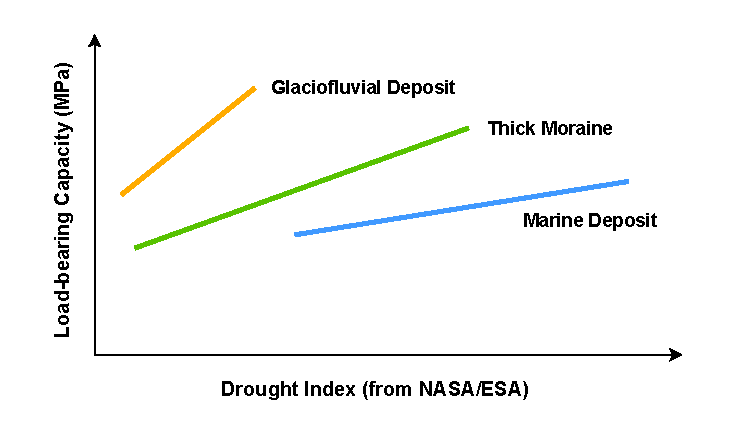
\includegraphics[width=0.7\linewidth]{figures/bæreevne_tørkeindex.pdf}
    \caption[Graph comparing load-bearing capacity to \acrshort{swi}]{Graph comparing load-bearing capacity to \acrshort{swi}, recreated from the task description [\hyperref[appendix:task_description]{Appendix \ref*{appendix:task_description}}]}
    \label{fig:load_to_swi_graph}
\end{figure}

While these studies highlight the feasibility of digital road classification, practical solutions for transport managers remain limited. Current industry practices often rely on experience-based assessments and manual planning, leading to inefficiencies and uncertainty. Although some digital tools have been developed to assist in forest road accessibility assessment, they are not universally applicable across different regions.

\section{Existing Solutions}
% Hva gjør transportledere nå? (spørsmål til usertesting maybe?)

One example is Harvester Seasons\footnote{\url{https://harvesterseasons.com/}}, developed by the Finnish Forest Center, which provides weekly forecasts of road conditions based on soil moisture, temperature, and snow depth. These forecasts use data from sources like \acrshort{nasa}'s \gls{smap} and \acrshort{esa}'s \Gls{sentinel-1} satellites to generate relative load-bearing predictions for winter and snow-free seasons [\hyperref[appendix:task_description]{Appendix \ref*{appendix:task_description}}]. While this tool offers valuable insights, it is limited to Finland and does not provide road condition data for Norway. As a result, it does not meet the needs of Skogkurs, which requires a solution tailored to Norwegian forest roads. This highlights the gap in available tools and the need for a localized approach that accounts for Norway’s specific terrain, climate, and forestry infrastructure.

The current process of scheduling operations for transport managers is based on weather conditions and road \gls{trafficability}. They plan operations either by necessity (e.g., during wet conditions) or by opportunity (e.g., in dry conditions). These decisions are informed by temperature-driven seasonality, regional precipitation patterns, and local knowledge. Additionally, transport lead times and road conditions are influenced by surface deposits and their \gls{permeability}, with difficult weather and reduced road \gls{trafficability} being major challenges in wood supply and transport management \cite{fjeld2023trafficability}. 

\section{Framework}

\textcolor{orange}{NOE TEKST}

\section{Project Organization}

\textcolor{orange}{NOE TEKST}

\section{Thesis Structure}

\textcolor{orange}{NOE TEKST}

\chapter{Requirements}\label{chap:requirements}

\textcolor{orange}{NOE TEKST}

This chapter presents the requirements provided the \gls{productowner}

This chapter presents a reflection on both the development process and the final product. It examines how the project evolved in relation to the original goals, highlighting what worked well, what could have been improved, and the challenges encountered along the way. The chapter discusses the choice of technologies, project management practices, and team collaboration. It also evaluates the effectiveness and limitations of the final solution, comparing it with existing alternatives and identifying unexpected findings. Broader considerations, such as sustainability and the role of AI in the project, are explored. Finally, the chapter outlines potential directions for future work and improvements to both the product and the project approach.


\section{Project Goals}

This section outlines the overall goal of the project, categorized into product goals, impact goals, and learning goals. Together, these objectives defines the purpose, intended outcomes, and the knowledge expected to be gained through the project process.

\subsection{Product Goals}\label{subsec:req:productgoals}

The primary goal of the project is to develop and test a \textbf{prototype system for fully digital modeling of forestry road load-bearing capacity under varying conditions throughout the year.} The solution will incorporate various geological and meteorological parameters, such as soil type and moisture, weather forecasts, and precipitation data, to generate an accurate classification of forest roads. This classification will be presented through an interactive map-based website. Furthermore, the system will prioritize ease of use, with an intuitive interface designed for transport managers, allowing them to make informed route choices based on real-time data and forecasts. 

\textcolor{orange}{DETTE UNDER ER IKKE NØDVENDIG HER}
The roads will be color-coded using a traffic-light system, where green indicates safe roads, yellow signals caution, and red highlights unsafe roads. The system will provide users with a forecast for road conditions at least a week into the future, enabling better planning and decision-making. 

\subsection{Impact Goals}\label{subsec:req:impactgoals}
% Bærekraft ?
\begin{itemize}
    \item Reduced uncertainty for transport managers when setting the routes using forest roads.
    \item To validate the prototype's feasibility and effectiveness by conducting tests with end-users, such as transport managers, to assess its performance and usability in real-world scenarios.
\end{itemize}

\subsection{Learning Goals}\label{subsec:req:learninggoals}
% Kanskje korte ned litt på dette
% Kanskje oppdatere med noe nytt?? WMS, GIS, osv.
\begin{itemize}
    \item Gaining insight in implementing interactive maps and geospatial data on web pages.
    \item Leveraging RESTful APIs for efficient data integration.
    \item Acquiring hands-on experience collaborating with real-world companies and products.
    \item Gaining experience working in a team environment, improving collaboration and communication skills.
    \item Conducting user tests and implementing feedback. 
    \item Developing a deeper understanding of the software development life cycle while actively practicing agile methodologies, like Scrum and Kanban.
    \item Enhancing application performance by implementing concurrency and optimizing parallel processing.
    \item Expanding proficiency in containerization techniques, particularly through hands-on experience with Docker.
    \item Implementing \Gls{openstack} deployment and configuration using Terraform for efficient infrastructure management.
    % Ikke ta med fra NTNU, heller referer
    \begin{comment}
    \item \textit{\textbf{From NTNU \cite{ntnu_idatg2900}:}}
    \begin{itemize}
        \item Has in-depth knowledge of a selected topic within the subject area.
        \item Has knowledge of research and development work within the topic.
        \item Can identify, formulate and solve a relevant engineering problem.
        \item Can apply knowledge and relevant results from research and development work to solve theoretical, technical and practical problems within the topic of the bachelor thesis and justify their choices.
        \item Can apply engineering methods and work methodically.
        \item Can document and disseminate engineering work.
        \item Can plan and carry out engineering work.
        \item Disseminates professional knowledge to various target groups both in writing and orally in Norwegian and English.
        \item Has insight into scientific honesty and understanding of ethical issues.
        \item Has insight into environmental, health, social and economic consequences of products and solutions within their field and can put these in an ethical perspective and a life cycle perspective.
        \item Integrates previously acquired knowledge and is able to acquire new knowledge in solving a problem.
    \end{itemize}
    \end{comment}
\end{itemize}

\section{Constraints}

\textcolor{orange}{NOE TEKST}

\subsection{Temporal Constraints}

\textcolor{orange}{NOE TEKST}

\begin{itemize}
    \item The set deadline for the final report is 20th of May.
    \item The presentation of the bachelor's thesis is scheduled for 4th or 5th of June.
\end{itemize}

\subsection{Product Constraints}

\textcolor{orange}{NOE TEKST}

\begin{itemize}
    \item The product requires a stable network connection to be used.
    \item The product uses \acrshort{html} 5, which requires newer versions of browsers.
    \item The product needs to be deployed either locally or on a server to run.
\end{itemize}

\begin{comment}
    \subsection{Legal Constraints}
% VET IKKE OM DETTE SKAL VÆRE MED
% ENDRE TIL NÅTID (THE PRODUCT COMPLIES WITH....) ?
\begin{itemize}
    \item The product must comply with the licensing terms and conditions of all third-party services, including map distributors, external APIs, and any code libraries, frameworks, or tools used in its development and deployment.
\end{itemize}
\end{comment}

\section{Project Tasks}
% VET IKKE OM DETTE SKAL VÆRE MED (KANSKJE FJERNE DELER ELLER PEK TIL PROSJEKT PLANEN)
The project aims to develop and test a prototype system for fully digital modeling of forest road load-bearing capacity under varying conditions throughout the year. The development process can be divided into the following areas:

\begin{enumerate}
    \item \textbf{Data Collection and Integration:}
    \begin{itemize}
        \item Decide and gather relevant geological and meteorological data, which may include:
        \begin{itemize}
            \item Superficial deposits, soil moisture, ground water, ground frost.
            \item Weather forecasts.
            \item Historical and real-time road conditions.
        \end{itemize}
        \item Identify and implement suitable data sources and APIs for continuous updates.
    \end{itemize}
    
    \item \textbf{Classification and Forecasting:}
    \begin{itemize}
        \item Develop a rule-based model to classify road conditions based on environmental factors.  
        \item Implement a traffic-light classification system (Green = Safe, Yellow = Caution, Red = Unsafe).  
        \item Extend the model to provide forecasted road conditions at least a week in advance.  
    \end{itemize}
    
    \item \textbf{Web-Based Visual and User Interface:}
    \begin{itemize}
        \item Design and develop an interactive map-based website for intuitive accessibility.
        \item Implement a GIS-based visualization with real-time updates and historical road condition tracking. 
        \item Ensure that the system is optimized for transport managers, with a user-friendly interface that allows efficient decision-making. 
    \end{itemize}
    
    \item \textbf{Testing, Validation and Refinement}:
    \begin{itemize}
        \item Evaluate the accuracy and usability of the system by testing with real-world data.
        \item Conduct user testing with transport managers or forestry stakeholders to assess the effectiveness of the interactive interface and forecasting capabilities.
        \item Incorporate potential user feedback.
    \end{itemize} 
    
    \item \textbf{Documentation and Future Work:}
    \begin{itemize}
        \item Provide detailed documentation of the system architecture, data sources, and model.
        \item Provide a detailed user guide of the product.
        \item Suggest potential improvements, such as machine learning model enhancements, additional data sources, mobile application integration, optimization, or further improvements of the app interface.
    \end{itemize}
\end{enumerate}

\section{Target Audience}

The primary target audience for this application is transport managers in the Norwegian forestry industry. They will use the application to plan routes and determine which forest roads should be used by drivers. Since the user group spans a wide age range, it is essential that the application is intuitive and easy to use, ensuring accessibility for all users regardless of their technical proficiency.

\section{Universal Design}

\textcolor{orange}{NOE TEKST}
\begin{comment}
    Kanskje ikke nødvendig med eget kapittel og kanskje ha det et annet sted? Passer med overgang fra Target Audience ^. SIDEN NOE OM DETTE IKKE BLE NEVNT AV SKOGKURS SÅ BURDE DET KANSKJE STÅ I DISCUSSION I STEDET.
\end{comment}

\section{Use Case}

Use cases provide a clear overview of what a system will and will not do. They enable effective scope management and incremental development, making them well-suited for agile methodologies \cite{jacobson_use_case}. 

This section will present the use case diagram of the system and provide an example of a use case specification.

\subsection{Use Case Diagram}
% DOBBELSJEKK AT SERVEREN IKKE SKAL KOBLES TIL USE CASENE I DIAGRAMMET
The use case diagram shows all interactions the user will have with the website. It also features the application server and its relationship with the external map servers.
\begin{figure}[h]
    \centering
    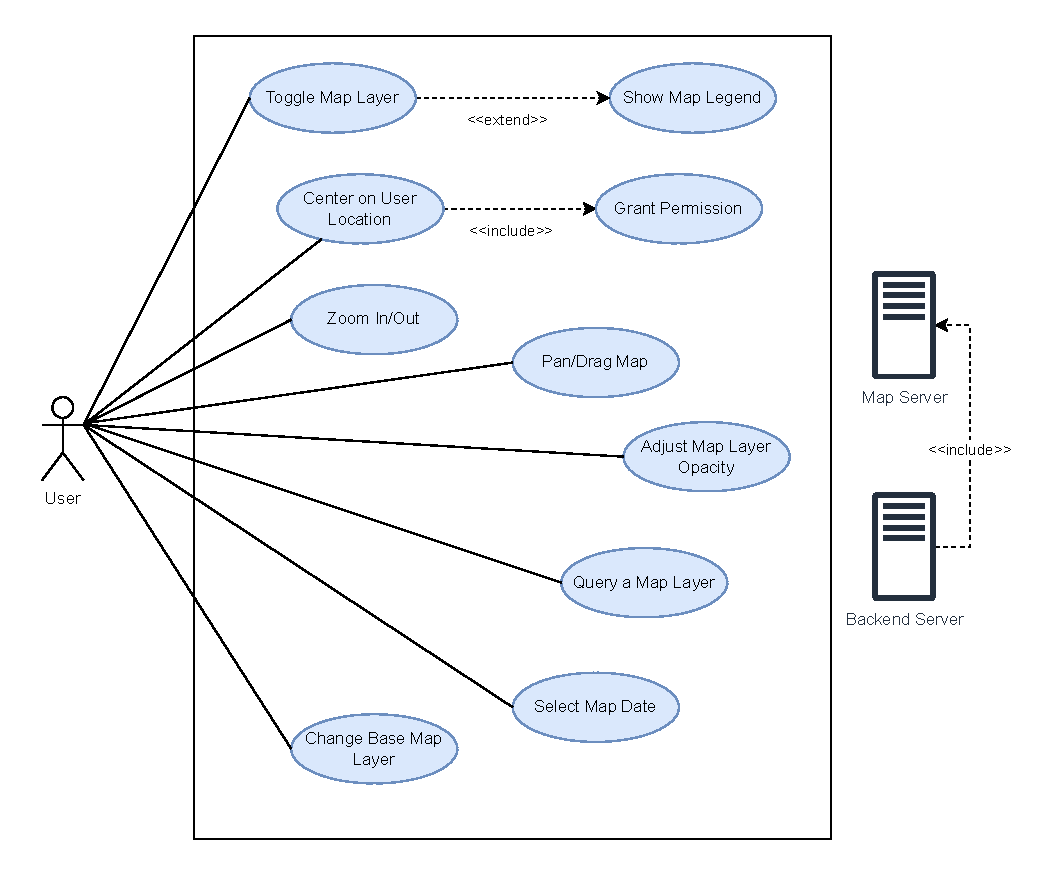
\includegraphics[width=1\linewidth]{figures/use_case_diagram.pdf}
    \caption{Use case diagram of system}
    \label{fig:use_case_diagram}
\end{figure}

\subsection{Actors}

\begin{itemize}
    \item \textbf{User:} The primary user of the website, typically transport managers in the forestry industry, who interact with the system to access relevant map and logistics data.
    \item \textbf{Backend Server:} The central server that the website communicates with to retrieve all necessary map data. It aggregates, processes, and refines data from external services before delivering it to the website.
    \item \textbf{Map Server:} External services that provide map data, either through a \Gls{wms}, \Gls{wfs}, or an \acrshort{api}, which the backend server integrates into the system.
\end{itemize}

\subsection{Use Case Specifications}

It is important to show how users interact with the system to achieve their goals. The use case specifications provide details of each use case and the basic path the user takes to achieve their goals while also capturing possible exceptions. 

A high priority use case for the website is the ability to toggle a map layer, which allows users to control the visibility of different layers. The use case specification for this functionality is shown in \hyperref[tab:use_case_toggle_layer]{Table \ref*{tab:use_case_toggle_layer}}. Additional use case specifications for other features can be found in \hyperref[appendix:use_case_specifications]{Appendix \ref*{appendix:use_case_specifications}}.

\begin{table}[h]
    \centering
    \begin{tabularx}{\textwidth}{|l|X|}
        \hline
        \rowcolor{gray!20}
        \textbf{Use Case Name} & Toggle Map Layer \\
        \hline
        \textbf{Actor(s)} & User \\
        \hline
        \textbf{Description} & The user can toggle specific map layers to control the visibility of different map layers. This functionality allows users to select from various map layers. The selected layer is then displayed, and relevant information is shown in the map legend sidebar. \\
        \hline
        \textbf{Priority} & High \\
        \hline
        \textbf{Pre-Condition(s)} & The user must have a stable internet connection and the website open. The website, server and external map servers must be deployed and running.\\
        \hline
        \textbf{Post-Condition(s)} & The map will be updated with the specific map layer that was toggled. The map legend will also be visible in the legend sidebar. \\
        \hline
        \textbf{Basic Path} &  
        \begin{enumerate}[label=,left=0pt]
            \item 1. User presses the map layer ("kartlag") button to open the map layer sidebar.
            \item 2. User clicks the toggle button for the specific map layer to toggle.
            \item 3. The system updates the map with the selected layer.
        \end{enumerate} \\
        \hline
        \textbf{Exception Path} & 
        \begin{enumerate}[label=,left=0pt]
            \item 0. User does not have a stable internet connection and can not connect to the website.
            \item 2a. Either the backend server or the map server is not responding, and no map data is received.
        \end{enumerate} \\
        \hline
    \end{tabularx}
    \caption[Use Case Specification: Toggle Map Layer]{Use case for toggling a map layer}
    \label{tab:use_case_toggle_layer}
\end{table}

\chapter{Technical Design}\label{chap:technicaldesign}

\begin{comment}
    # Universal Design (Universal Utforming)
    # OpenLayers vs Leaflet (or others)
    # Openlayers TileWMS vs ImageWMS (optimalisering av kartet)
\end{comment}
\textcolor{orange}{NOE TEKST}

\section{System Architecture}\label{sec:systemarchitecture}

% client-server model, microservices, layers of the application ? 
\textcolor{orange}{NOE TEKST}

\section{Data Flow} % e.g., how user requests move through the system).

\textcolor{orange}{KANSKJE TEMP LOKASJON}

\section{Sequence Diagram}
\begin{figure}[h]
    \centering
    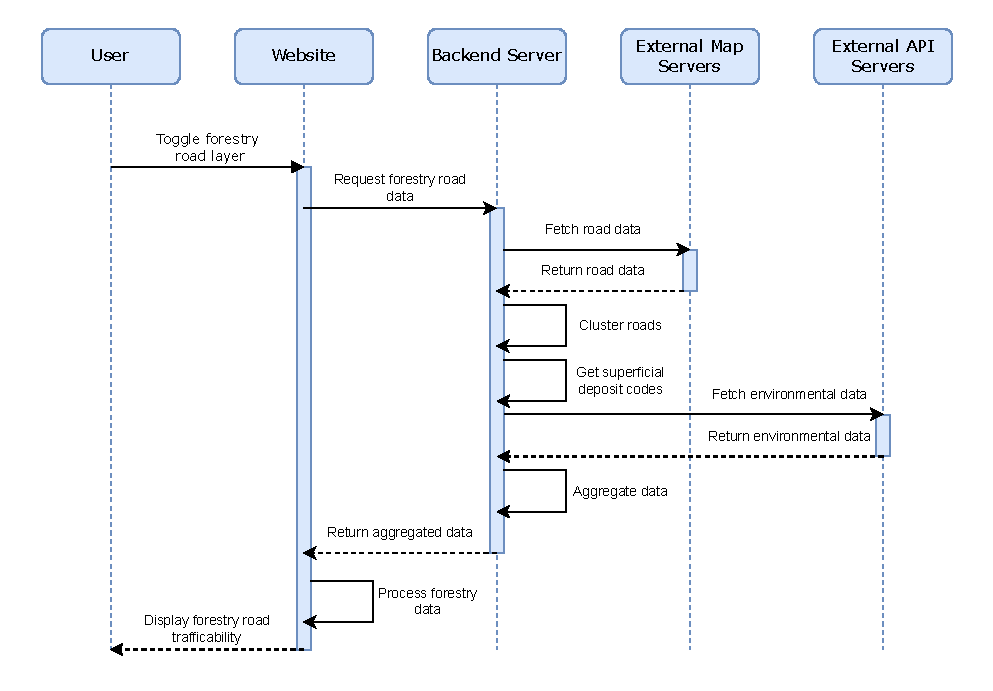
\includegraphics[width=1\linewidth]{figures/sequence_diagram.pdf}
    \caption{Sequence diagram of forestry road map layer}
    \label{fig:sequence_diagram}
\end{figure}

\hyperref[fig:sequence_diagram]{Figure \ref*{fig:sequence_diagram}} shows the sequence diagram for when the user toggles the forestry road map layer. The whole sequence consists of these steps:
\begin{enumerate}
    \item \textbf{Toggle forestry road layer}: The user toggles the forestry road map layer on the website.
    \item \textbf{Request forestry road data}: The website sends a request to the backend server for the necessary data within the visible map area.
    \item \textbf{Fetch road and weather data}: The backend server, acting as a proxy, fetches the required road and weather data from external map servers.
    \item \textbf{Return road and weather data}: The map servers return the requested road and weather data.
    \item \textbf{Aggregate data}: The backend server aggregates the data into a single payload.
    \item \textbf{Return aggregated data}: The backend server sends the aggregated data back to the website.
    \item \textbf{Process forestry data}: The website processes the data and determines the trafficability of roads within the visible map area.
    \item \textbf{Display forestry road trafficability}: The forestry road layer, including trafficability, is rendered on the user's map.
\end{enumerate}

\section{Website}

The website serves as the user interface of the system, allowing users to visualize and interact with data related to forestry road conditions and weather-based forecasts using a dynamic map.

The system follows a client-server architecture, where the website acts as a client and communicates with a backend server via a REST API. The processing of meteorological and geological data is handled on the server side. The frontend is responsible for requesting data, rendering maps, and presenting relevant information to the user.

The classification of road trafficability is performed on the client side, as the website allows users to dynamically adjust thresholds for certain meteorological and geological parameters. Normally, this would be handled entirely by the backend server, but in order to provide immediate feedback when the user changes these thresholds, the classification logic is implemented in the frontend. This hybrid approach ensures a responsive user experience while keeping the most computationally expensive operations on the server.

The interaction between the website and the server is stateless, meaning that each request is independent and contains all the information needed to process it. This architectural choice improves system robustness and simplifies both development and deployment, particularly when it comes to scaling.

A central component of the website is its interactive map interface, which displays spatial data such as forestry road networks, map layers, and calculated trafficability classifications. The map is rendered dynamically in the browser using client-side resources, and data is loaded based on the user’s current viewport and zoom level. This approach ensures efficient data usage and good performance, even when dealing with large or detailed geographic datasets.

The website is implemented as a single-page application (SPA), where all rendering and interface updates occur dynamically without full page reloads. This enables smooth interaction and better performance, as only relevant parts of the page are updated via the Document Object Model (DOM). \acrshort{html} 5 is required for full functionality, and the system relies on an active internet connection to fetch data from the server and external services. While the system is primarily intended for desktop and laptop use, it also runs on mobile devices, though the \acrshort{ui} is not optimized for smaller screens.

Choosing to implement the frontend as a web application provides several benefits. It ensures accessibility across a wide range of devices without the need for local installation, making the tool usable both in office environments and in the field.

Overall, the design of the website emphasizes a clean separation of concerns, efficiency in data handling, and accessibility, which together form a robust and user-friendly frontend component for the system.

\subsection{Road Classification}

\textcolor{orange}{
Blablabla noe \autoref{fig:forestryroadclassification}
}

\begin{figure}[h]
    \centering
    \centerline{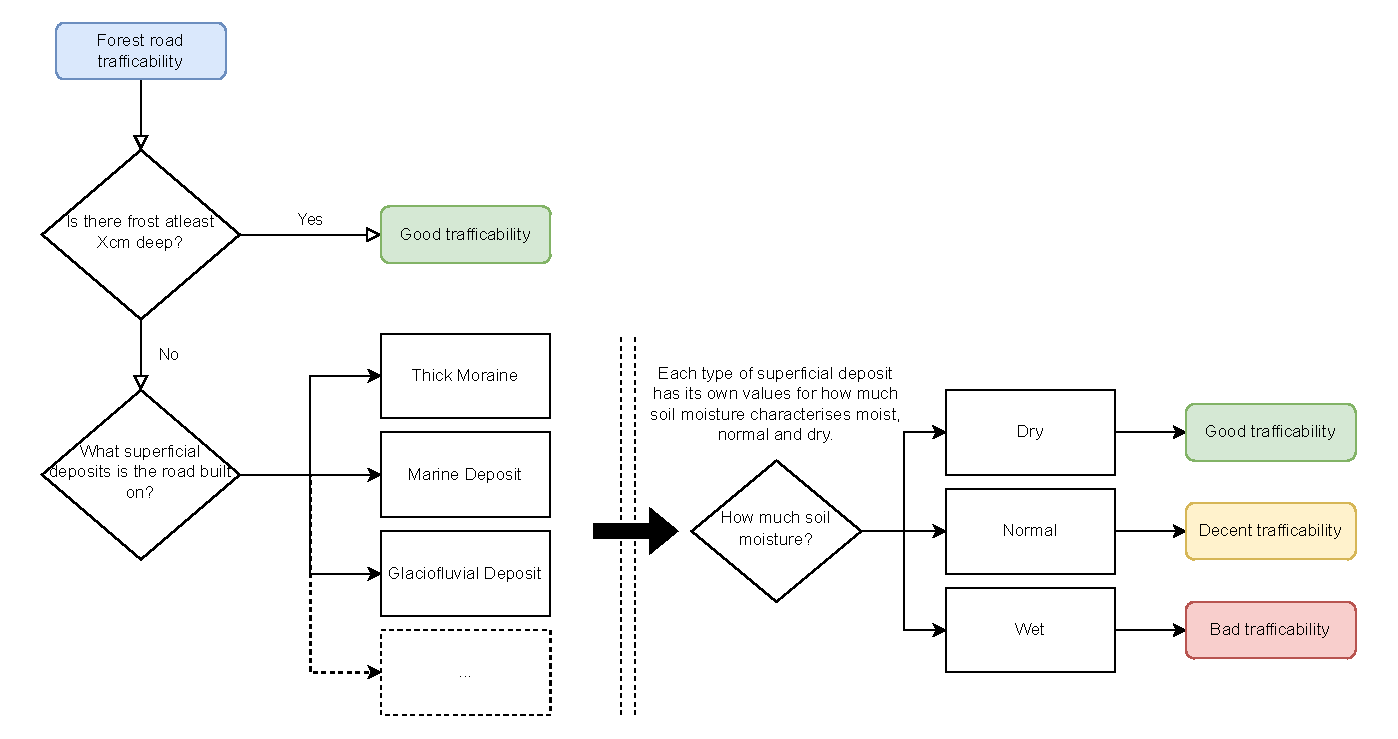
\includegraphics[width=1.2\linewidth]{figures/roadclassification.pdf}}
    \caption{Diagram visualizing the forestry road classification}
    \label{fig:forestryroadclassification}
\end{figure}

\subsection{Folder Structure}

\textcolor{orange}{NOE TEKST}
\begin{figure}[h]
    \centering
    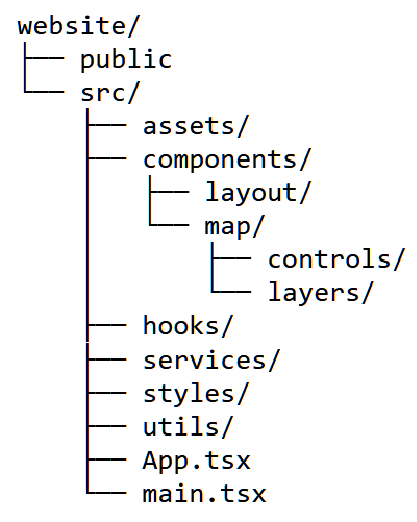
\includegraphics[width=0.5\linewidth]{figures/website_folder_structure.pdf}
    \caption{Folder structure of the website}
    \label{fig:website_folder_structure}
\end{figure}

\section{Server}

\textcolor{orange}{NOE TEKST}

\subsection{Forestry Road Processing}

\subsection{Proxy}


% Multiple map services were used in this project to ultimately determine the trafficability of forestry roads. Retrieving data from WMS and WFS was made easy with OpenLayers as it includes functions for this. 


\subsection{Folder Structure}



% ANDRE DIAGRAM? sequence diagrams, component diagrams, etc.
\chapter{Development Process}

\section{Code Repository}
% Github Organization and repos
All code and project-related resources are stored on GitHub under a dedicated organization\footnote{\url{https://github.com/skogkursbachelor}}. Each component of the system, as well as supporting documentation, is maintained in its own repository. This modular structure facilitates collaboration and version control throughout the development process.

An overview of the repositories and their respective purposes is shown in \hyperref[tab:github_repositories]{Table \ref*{tab:github_repositories}}.

\begin{table}[h]
    \centering
    \begin{tabular}{l|l}
        \hline
        \textbf{Repository} & \textbf{Description} \\
        \hline
        server & The code for the backend server. \\
        website & The code for the website. \\
        \hline
        meetingminutes & A backup of all meeting minutes. \\
        diagrams & A backup of all diagrams. \\
        thesis & A backup version of the thesis. \\
        projectplan & A backup version of the project plan. \\
        \hline
    \end{tabular}
    \caption{Overview of all GitHub repositories\footnotemark}
    \label{tab:github_repositories}
\end{table}
\footnotetext{\url{https://github.com/orgs/skogkursbachelor/repositories}}

\section{Time Tracking}
All project work was tracked using the self-hosted time tracking service Traggo\footnote{\url{https://traggo.net/}}. Traggo tracks work by tags making it easy to get an overview of time spent on different tasks.

\begin{table}[h]
    \centering
    \begin{tabular}{c|c|c|c}
        \hline
        \textbf{Month} & \textbf{Bjørnsen} & \textbf{Houmb} & \textbf{Total} \\
        \hline
        January  & 61h 39m  & 62h 58m  & 124h 37m \\
        February & 80h 6m   & 79h 17m  & 159h 24m \\
        March    & 88h 4m   & 88h 20m  & 176h 24m \\
        April    & 35h 36m  & 31h 18m  & 66h 54m \\
        May      &        &        &        \\
        \hline
        Total & & & \\
        \hline
    \end{tabular}
    \caption{Tracked time by month and group member}
    \label{tab:tracked_time_by_month_member}
\end{table}

% Skriv mer om time fordeling, f.eks. hvorfor mer timer i mars enn januar etc.
\hyperref[tab:tracked_time_by_month_member]{Table \ref*{tab:tracked_time_by_month_member}} shows the total time of work for each month and each group member.

% KANSKJE IKKE TA SKJERMBILDE, LAG HELLER CHART MED LATEX f.eks. (pfg-pie).
\begin{figure}[h]
    \centering
    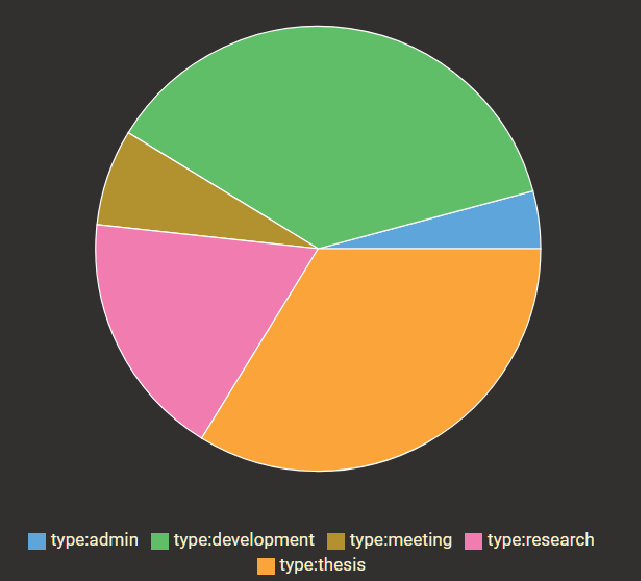
\includegraphics[width=0.5\linewidth]{figures/time_tracking_by_type.pdf}
    \caption{Pie chart of time spent in total per work type}
    \label{fig:time_tracking_by_type}
\end{figure}

% SKRIV OM TIDSFORDELING FOR DE FORSKJELLIGE OPPGAVENE (THESIS, DEV, osv.)

To provide an overview of the project timeline, a Gantt chart was created, highlighting the different sprints and key milestones. A more detailed table of all dates referenced in the Gantt chart can be found in \hyperref[appendix:project_plan]{Appendix \ref*{appendix:project_plan}}.

\section{Gantt Diagram}
\begin{figure}[h]
    \centering
        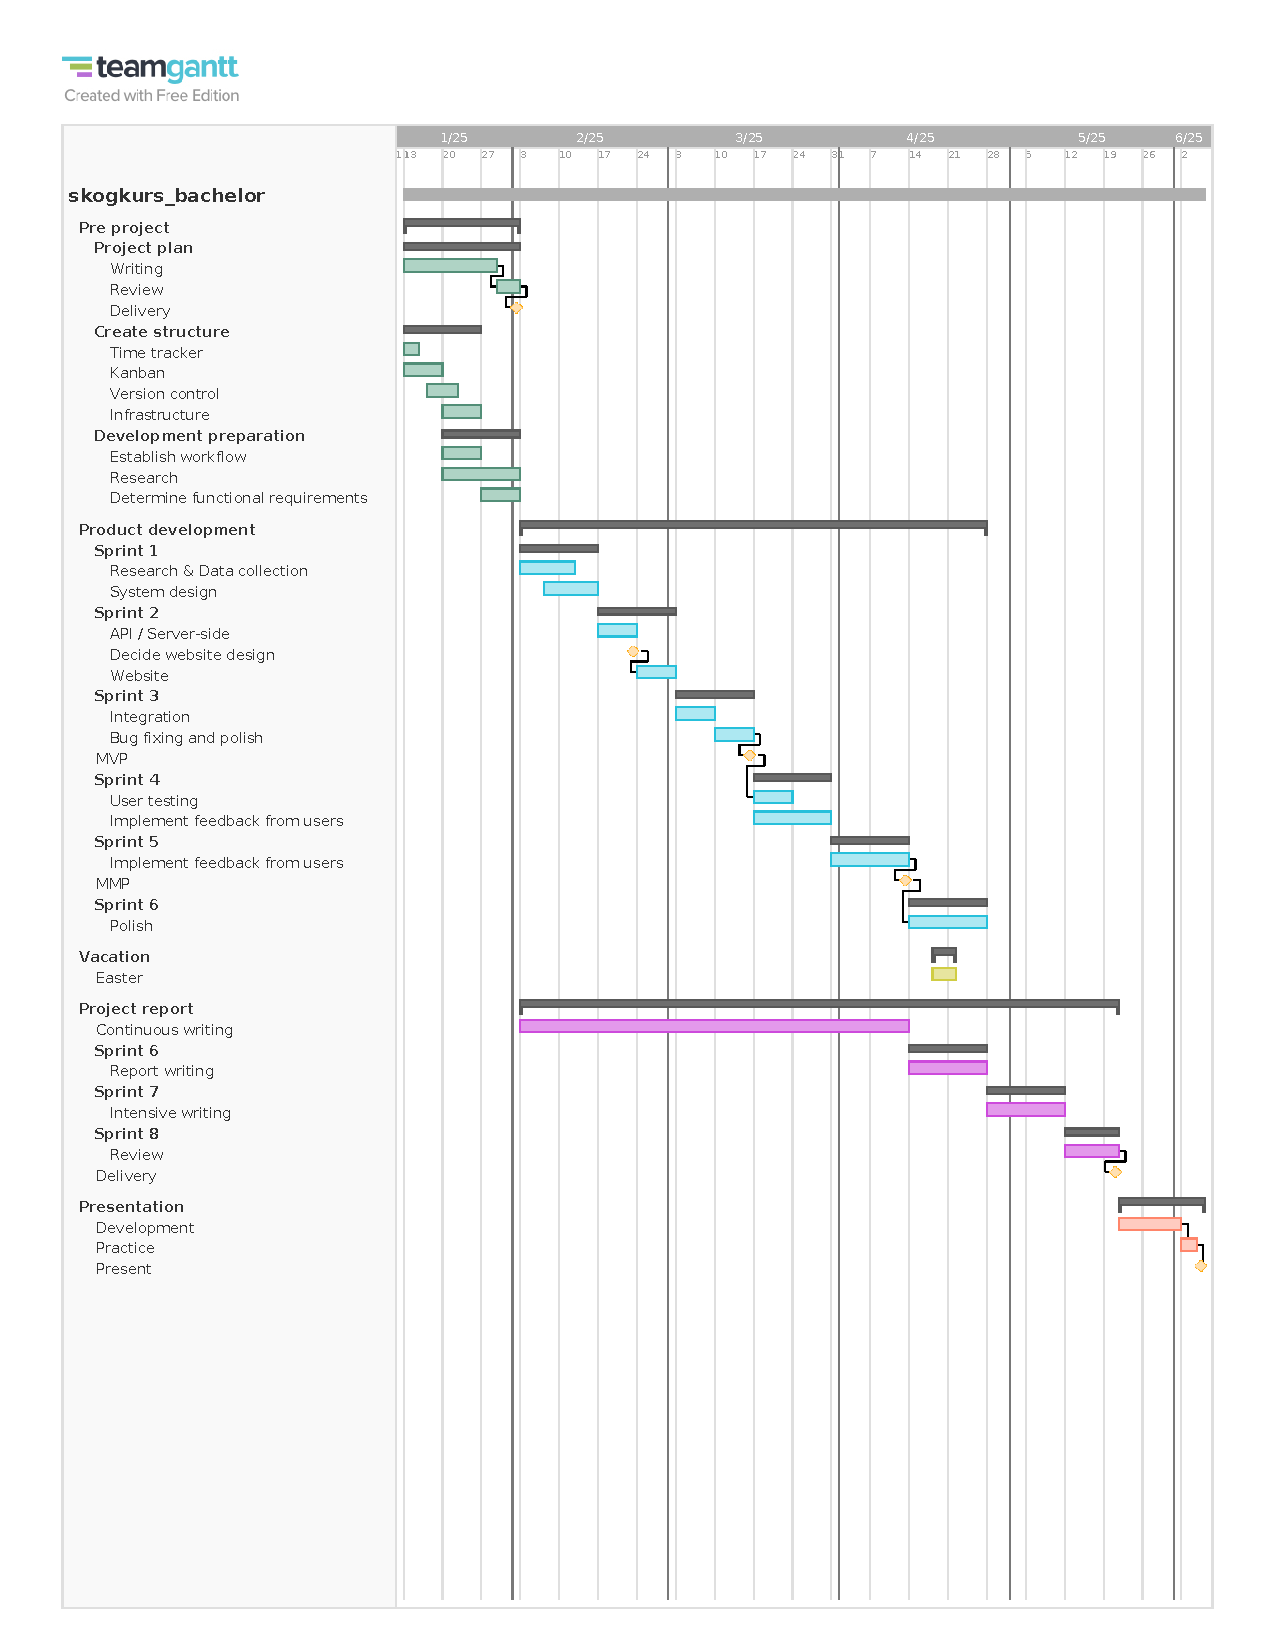
\includegraphics[width=1.0\linewidth, trim=0 60mm 0 20mm, clip]{figures/skogkurs_bachelor_gantt.pdf}
    \caption{Gantt diagram of the project}
    \label{fig:gantt_diagram}
\end{figure}

\section{Software Development Lifecycle Model}

For this project, the team needed to select an appropriate Software Development Lifecycle (\acrshort{sdlc}) model. Key factors considered in this decision included the clarity and flexibility of the requirements, team size, project timeline, product delivery goals, and prior experience \cite{sdlc_model}. 
\\ \\
The requirements provided by the Product Owner are intentionally ambiguous and flexible, allowing the team to prioritize the few fixed requirements upfront while iteratively refining the flexible ones over time. The team is composed of two members with similar experience levels, enabling close collaboration and effective decision-making. With a short project timeline of four months, a structure of 2-week sprints aligns perfectly with Scrum's iterative and adaptive approach, ensuring steady progress and regular opportunities for feedback. 
\\ \\
Since our project lacks clearly defined requirements and requires ongoing collaboration with the Product Owner, Scrum was the best fit for our team and project. Traditional methodologies like Waterfall were not suitable, as they rely on fixed requirements and a linear development process, which would limit our flexibility. Extreme Programming (XP), while valuable for high-collaboration environments with strict engineering practices like pair programming and test-driven development, was not fully suitable as our project does not emphasize these practices to the same extent \cite{extreme_programming}. Similarly, Lean development focuses on minimizing waste and maximizing efficiency but is less structured in terms of iterative planning, which we need to manage evolving requirements effectively \cite{lean_programming}. By adopting Scrum, we can iteratively refine requirements and adapt to changes throughout development \cite{sdlc_model}. To implement Scrum effectively, several key practices will be integrated into our workflow \cite{scrum_guide}.

\begin{itemize}
    \item \textbf{Sprint Meetings:} The project will be divided into 2-week sprints. At the start of each sprint, sprint meetings will include sprint planning, reviews, and retrospectives. During the planning phase, the team will select tasks from the product backlog to form the sprint backlog for the upcoming sprint. The review phase will focus on assessing progress and determining whether adjustments to the product backlog are needed. The retrospective phase will identify areas for improvement in the Scrum process itself.
    \item \textbf{Daily Scrum Meetings:} Short daily meetings will be conducted to discuss the progress of ongoing tasks, identify potential obstacles, and ensure alignment between team members.
    \item \textbf{Scrum Master:} Given that the team consists of only two members, we have decided to share the role of Scrum Master. Both members are responsible for ensuring adherence to the Scrum framework and continuously working to improve team efficiency. This collaborative approach allows us to maintain flexibility while upholding Scrum principles throughout the project.
    \item \textbf{Kanban:} To complement Scrum and further enhance workflow visibility, the team will utilize a Kanban board to track and manage tasks on GitHub. The Kanban board will consist of columns representing different stages of the workflow, such as Product Backlog, Sprint Backlog, In Progress, In Review, Done, and Discarded.
\end{itemize}

\section{Sprints}
% Kanskje peke til vedlegg?
% Sammenlign med det som står over, ta med sprint planning, reviews og retrospective
\subsection{Sprint 1: 03.02.2025 - 14.02.2025}
\begin{comment}
- Fyll ut Product Backlog
- Undersøke forskjellige datakilder for kart- og geodata
    - Senorge (https://api.nve.no/doc/gridtimeseries-data-gts/)
	- Geonorge (løsmasser, skogsbilveg)
	- NGU
	- NIBIO 
- System Design (?)
    - Sequence Diagram
	- Use Case Diagram
	- Activity Diagram
	- Component Diagram
\end{comment}
The primary objectives of the first sprint were to populate the product backlog for the entire project and to research potential sources of map and weather data. Data sources that were already under consideration or recommended by the product owner included:
\begin{itemize} 
    \item Senorge
    \item Geonorge
    \item NGU
    \item NIBIO
\end{itemize}

From these source the map layers for superficial deposits, frost depth, soil moisture, and forestry roads were selected using a WMS.

Additionally, the sprint included the development of the initial system diagrams. 

With the primary tasks completed, the remaining time in the sprint was used to begin developing the website. This included familiarizing with the OpenLayers library and testing the integration of the selected map layers.

\subsection{Sprint 2: 17.02.2025 - 28.02.2025}
\begin{comment}
## Hvordan gikk forrige sprint
- Fikk gjort alt i sprint back-loggen
- Bestemte oss for å begynne å utvikle nettsiden for å få testet ut de forskjellige kartlagene / geodataene
## Hva gjøre i løpet av neste sprint
- Implementere datakildene inn i nettsiden:
	- Markfuktighet
	- Grunnvann
	- Teledyp
	- Skogsbilveger
\end{comment}
This sprint was mainly focused on implementing the website and the required features. The integration of each map layer was finished and an initial version of the website was shown to the product owner.  

\subsection{Sprint 3: 03.03.2025 - 14.03.2025}
\begin{comment}
## Hvordan gikk forrige sprint
- Fikk laget ferdig en versjon vi var fornøyd med å vise frem til produkteier
- Fikk implementert disse datakildene:
	- Løsmasser
	- Teledyp
	- Markfuktighet
	- Jordfuktighet (historisk)
	- Skogsbilveger
## Hva gjøre i løpet av neste sprint
- Få prognose av jordfuktighet (open-meteo, hvis ingen bedre løsning)
- Lage en måte for å konvertere open-meteo data til geojson (eller andre format som passer til openlayers)
- Lage klassifiseringssystemet av skogsbilveger (rød, gul, grønn)
\end{comment}
In this sprint the objective was to start creating the classification system for forestry roads. 

\subsection{Sprint 4: 17.03.2025 - 28.03.2025}
\begin{comment}
## Hvordan gikk forrige sprint
- Å implementere open-meteo som kilde ble nedprioritert i forhold til klassifiseringen av skogsbilveg.
- Fikk begynt på skogsbilveg klassifiseringen, men på grunn av eksamen i et annet fag, ble det ikke ferdig.
- Fant en annen kilde hos MET for jordtemperatur og -fukt, m.m., men kun 3 dagers prognose.
- Gikk ned fra 40-45 timer på 2 uker til ca 20 timer som viser at fokuset ikke var fullt på bacheloroppgaven.
- Fikk satt opp første utkast av strukturen til rapporten og notert ned smått på enkelte kapittel.
## Hva gjøre i løpet av neste sprint
- Fullføre klassifiseringen av skogsbilvegene og samhandlingen med andre kartlag.
- Implementere selve klassifiseringsfunksjonene i backend.
- Fortsette med rapporten.
- Den planlagte brukertesten av MVP-en (ifølge Gantt-diagrammet) blir flyttet til neste sprint.   
\end{comment}

\subsection{Sprint 5: 31.03.2025 - 11.04.2025}

\subsection{Sprint 6: 14.04.2025 - 25.04.2025}

\subsection{Sprint 7: 28.04.2025 - 09.05.2025}

\subsection{Sprint 8: 12.05.2025 - 20.05.2025}

\section{Minimum Viable Product}
A Minimum Viable Product (MVP) is a concept that focuses on learning about customers with minimal effort. An MVP is an early version of a product designed to test whether customers will use or buy it, often taking the form of a simple prototype, landing page, or manually operated service. The key benefit of an MVP is that it allows teams to validate ideas early, minimizing wasted effort on products that may not succeed \cite{agile_alliance_mvp}. 

During the development of the website, we conducted user testing to gain insights into how the target audience (transport managers) would interact with the product and identify any missing features or necessary improvements. For the MVP, we prioritized implementing the core functionalities we believed users would need, as illustrated in the use case diagram in \hyperref[fig:use_case_diagram]{Figure \ref*{fig:use_case_diagram}}. Further details about the user testing process and findings are discussed in a later chapter.

\section{Minimum Marketable Product}

A Minimum Marketable Product (MMP) is the next step after an MVP in product development. While an MVP focuses on testing assumptions and user preferences, an MMP includes essential features that meet customer needs, provide a good user experience, and generate business value. It is designed to launch quickly with must-have functionality, avoiding unnecessary features that add complexity without value. The MMP approach involves refining the product to only what is essential for success. Typically, teams first develop MVPs to gather insights, then use these findings to build an MMP ready for general release. In agile development, combining MVPs and MMPs helps streamline product evolution while minimizing risk and unnecessary work \cite{wanner_mmp}. 

After conducting the user testing we used the feedback given to improve the product and ultimately reaching an MMP. 

\begin{comment}
UTFORDINGER I PROSESSEN:
- Eksamen i systemtenkning (?)

\end{comment}
\chapter{Implementation}
\begin{comment}
    - Github? forskjellige repo?
    - External data / sources used for map, etc.
\end{comment}

\section{Website}
This section contains an overview of the implementation of the website.
\begin{comment}
    - Typescript & React (vite/template, code structure?)
        - Template: npm create vite@latest myapp -- --template react-ts
    - OpenLayers
    - GUI-elements
    - Map layers and legends
    - Forestry road vector layer
    - Datepicker / temporal aspect of map layers
\end{comment}
\subsection{Wireframe} % Vet ikke om dette burde være et annet sted?
A wireframe of the website was made to agree on the layout of the website and the required features. \hyperref[fig:wireframe_website_sidebars_closed]{Figure \ref*{fig:wireframe_website_sidebars_closed}} shows the basic layout of the website including the map and the date picker. In \hyperref[fig:wireframe_website_sidebars_opened]{Figure \ref*{fig:wireframe_website_sidebars_opened}} it shows the sidebars for both enabling map layers and their legends. Additionally it shows a layer being enabled and querying that feature for additional information.
\begin{figure}[h]
    \centering
    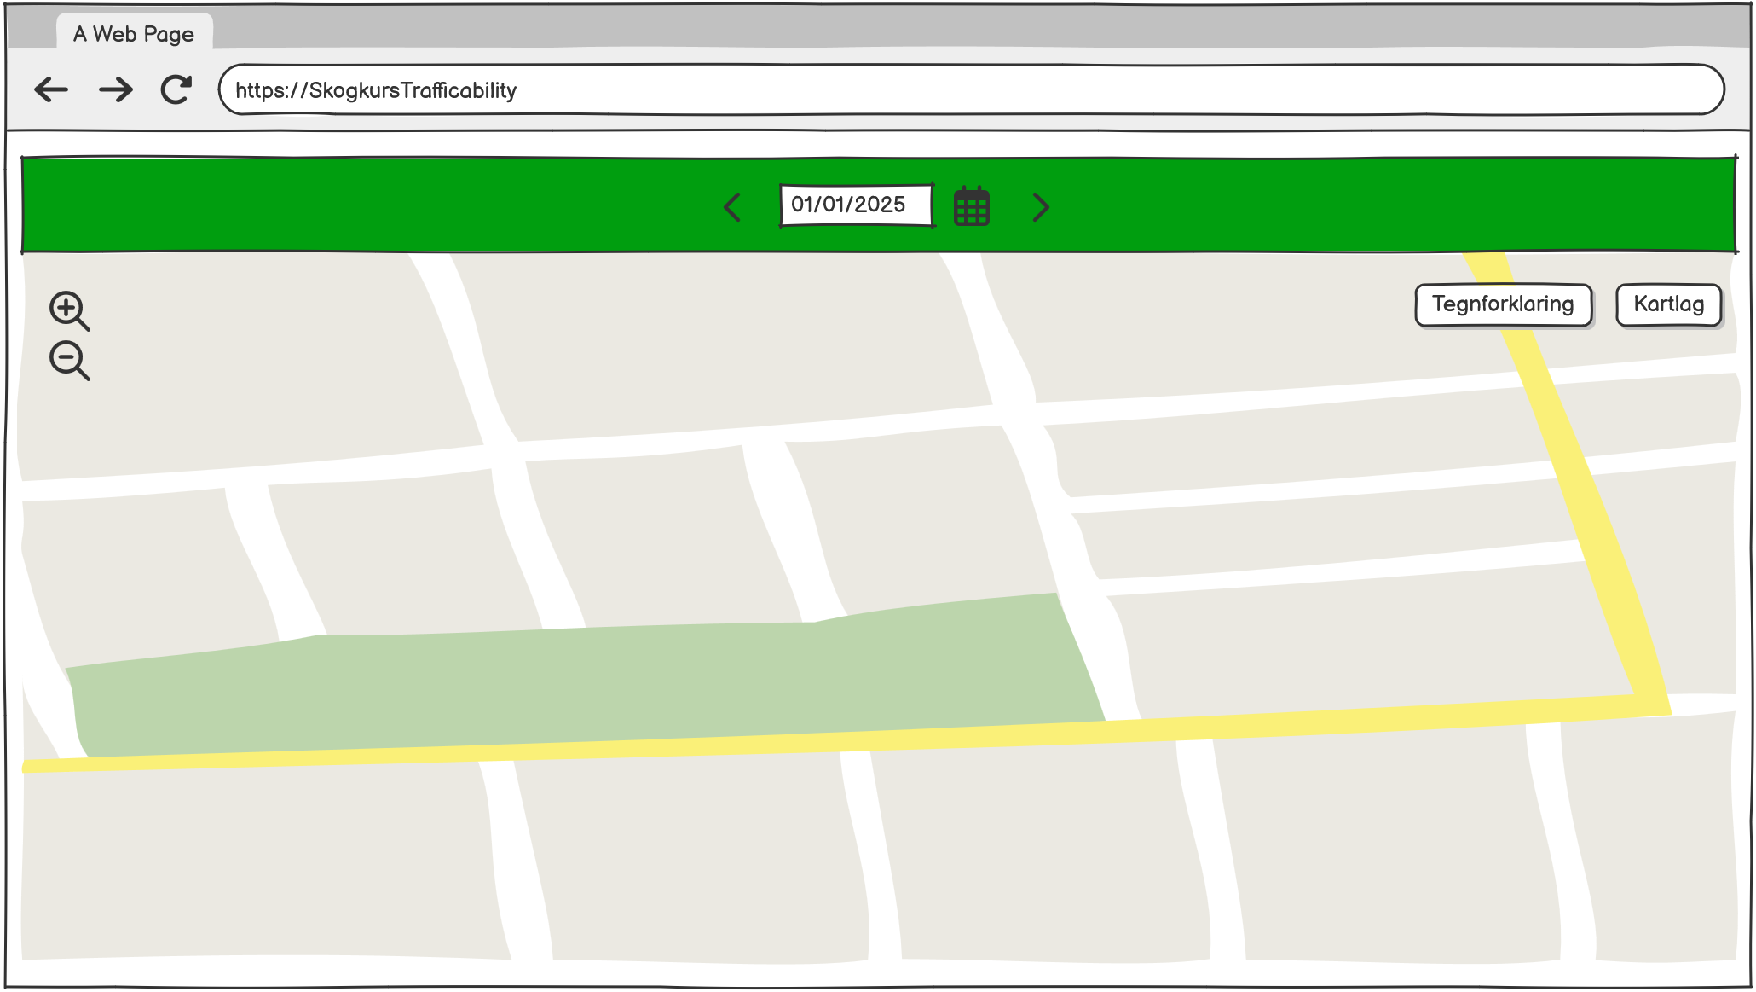
\includegraphics[width=0.6\linewidth]{figures/wireframe_website_sidebars_closed.pdf} 
    \caption{Wireframe of the website with no map layer enabled}
    \label{fig:wireframe_website_sidebars_closed}
\end{figure}

\begin{figure}[h]
    \centering
    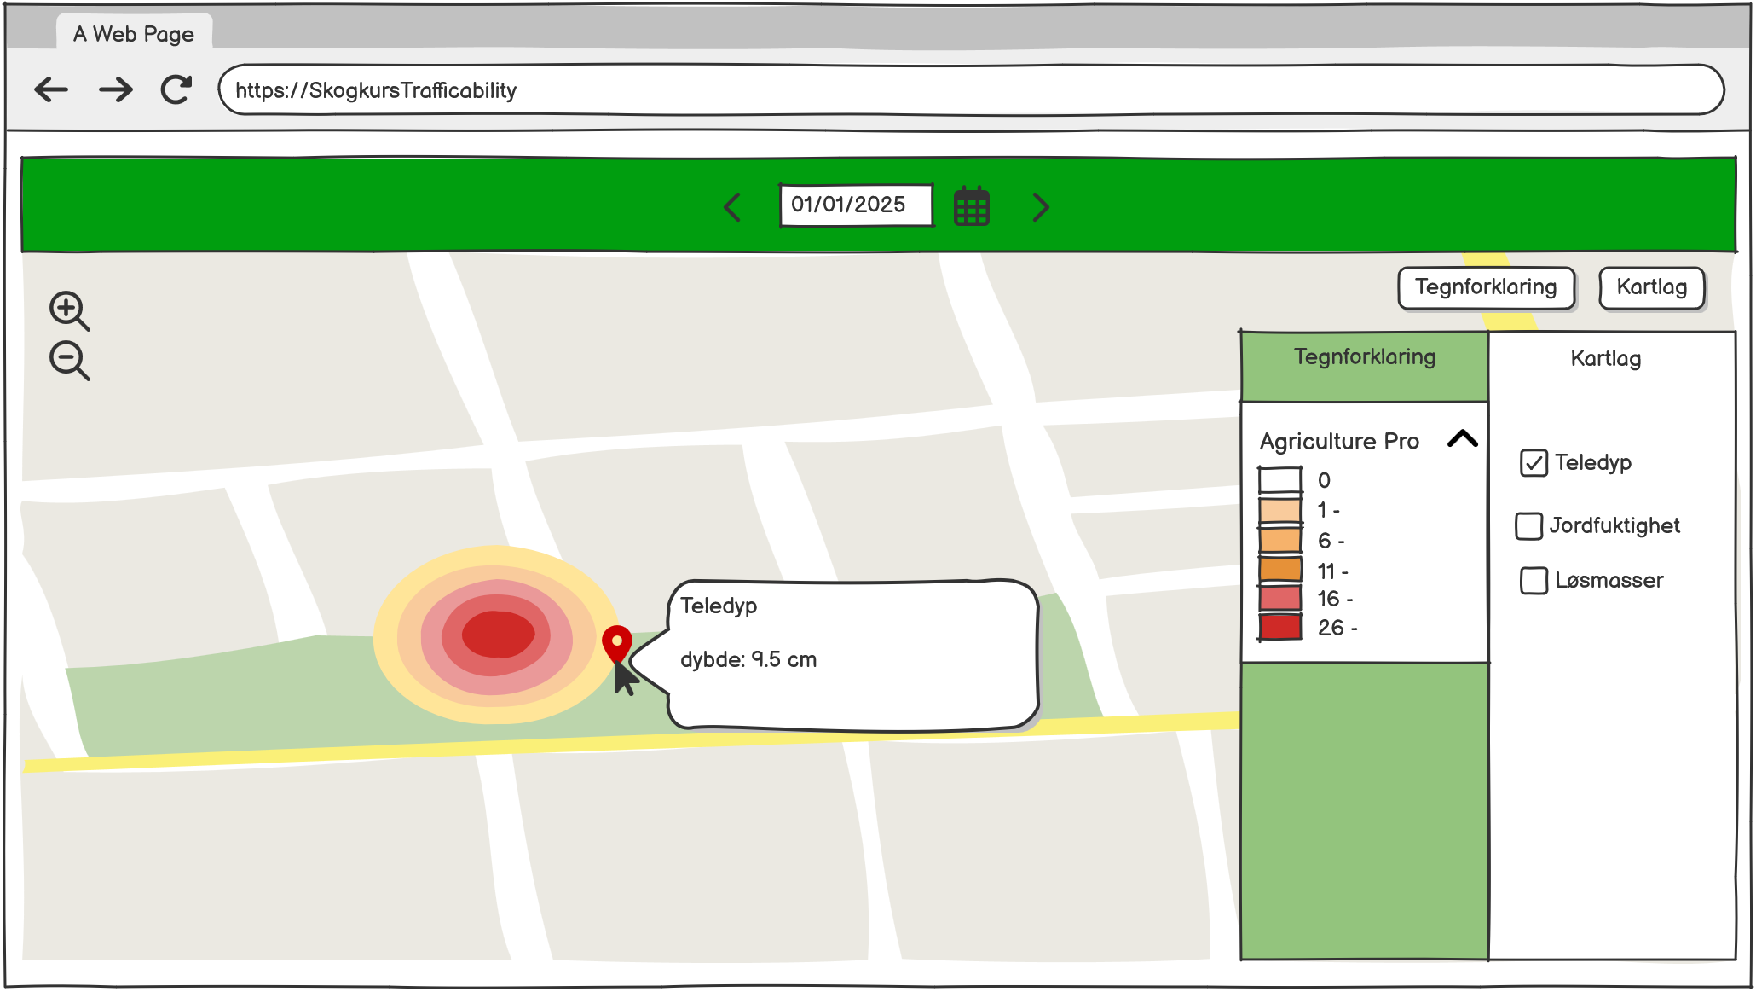
\includegraphics[width=0.6\linewidth]{figures/wireframe_website_sidebars_opened.pdf}
    \caption{Wireframe of the website with a map layer enable}
    \label{fig:wireframe_website_sidebars_opened}
\end{figure}


\subsection{UI Components}
\begin{figure}[h]
    \centering
    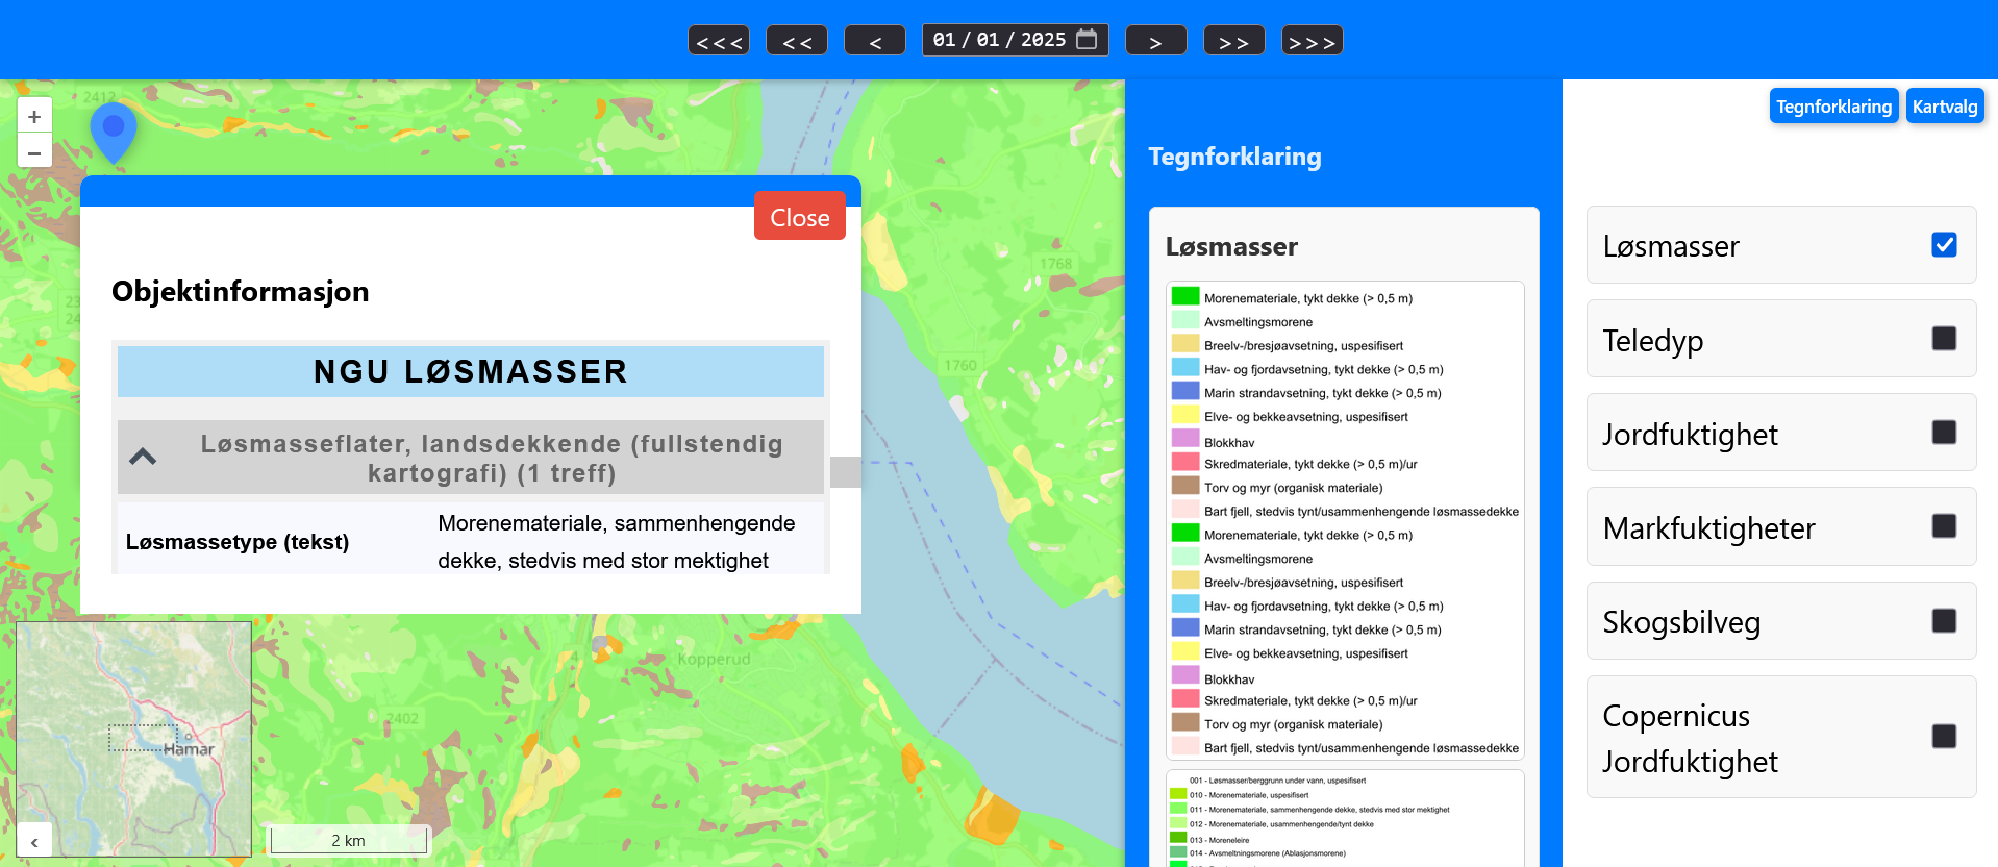
\includegraphics[width=1\linewidth]{figures/website_layout_v1.pdf}
    \caption{Early version of website}
    \label{fig:website_layout_v1}
\end{figure}

\subsection{Component State} % eller state management?

\subsection{Map Layers}

\subsection{Date Picker}
The date picker is used to change the current date of the data shown on the map. This lets the user see historical and forecast data. The component consists of an \acrshort{html} date input element and buttons to change the date by day, week or year. When the user changes the date, all enabled map layers will be updated with the new date and displayed on the map as long as they have data from that specific date.

\subsection{Trafficability Algorithm} % Processing Algorithm?

% 

\section{Server}

The backend server consists of TWO/THREE endpoints: a proxy for \Gls{wms} services, a query aggregator and the forestry road NOE. 
% Generelt om Server
The backend server is written in Go (REF/GLOSS) and designed as a REST API (REF/GLOSS). 

\begin{table}[h]
    \centering
    \begin{tabular}{l|l}
        \hline
        \textbf{Library} & \textbf{Description} \\
        \hline
        joho/godotenv & Loads environment variables from .env files. \\
        rs/zerolog & Zero Allocation Logger. \\
        tidwall/rtree & An R-tree implementation for spatial querying. \\
        twpayne/go-geom & Efficient geometry types for geospatial applications. \\
        twpayne/go-proj & Transformation between different coordinate systems. \\
        twpayne/go-shapefile & Native Go reader for ESRI Shapefiles \\
        \hline
    \end{tabular}
    \caption{Overview of used Go libraries}
    \label{tab:go_libraries}
\end{table}

\begin{comment}
\item[Implementation:] Here you should describe the more technical details of the solution. Which tools were used (programming languages, libraries, IDEs, APIs, frameworks, etc.). It is a good idea to give some code examples. If class diagrams, database models etc. were not presented in the technical design chapter, they can be included here.
    - Golang (libraries?)
    - Source of map layers/ legends (endpoint, etc.)
    - Proxy
    - Algorithm for trafficability of forest roads
\end{comment}
\subsection{Forestry road NOE} % Algorithm? Handler?

\subsection{Proxy}\label{subsec:proxy}

As described in Section \ref{sec:systemarchitecture}, we wanted a clean architecture where all requests went through the backend server. 

% Hvordan proxien funker
% Hva er effekten av en slik proxy
    % slik at clienten snakker med website, og website snakker med verdenen gjennom backend serveren

\subsection{Optimization}
% Nevn lang response time for brukeren ved "TOGGLING" av forestry roads
blabla During development the forest road retrieval algorithm was processing for too long, so some optimization had to be made.

\subsubsection{Spatial querying}

% Rtree ble brukt for å ha effektiv querying av spatial data. Skulle egentlig bruke querying av WMS, men fant fort ut at det var urealistisk med så mange requests. I tilegg var dataen om løsmasser tilgjengelig under NLOD, så en in-memory løsning ville funke. R-tree ble derfor valgt ettersom det er en effektiv datastruktur for querying of spatial data. Implementasjonen bygger et r-tree fra SHAPE filer.

\subsubsection{SeNorge}

The backend would initially query the SeNorge API once for every road, which would quickly overload the API server leading to long processing times. Additionally, the SeNorge API would not accept multiple coordinates within each grid-cell. SeNorge uses a grid system to divide Norway into \qty{1}{\kilo\meter\squared} cells, and calculate all their climate projections as an average within each cell \cite{senorge_omvannkart}. 

Lacking documentation of how the grid-cells were initially declared, in addition to a deprecated service for transforming coordinates to cell indexes, prompted further investigation into the SeNorge grid-cells. Findings showed that each grid-cell had borders that lined up with the UTM zone 33N projection system, where the latitude and longitude of each grid intersection were a multiple of \qty{1000}{}. In other words, each grid is centered on a UTM coordinate that is a multiple of $\qty{1000}{}\pm\qty{500}{}$.

The findings made it possible to cluster the forest roads into their closest SeNorge grid-cell, without explicitly knowing which grid-cell was closest. The coordinate of the cluster center could then be used to send a singular request to the SeNorge API, drastically increasing the amount of roads that could be processed at once. Listing \ref{lst:clusterforestroads} shows the implementation of the clustering, where the forest roads are clustered into a sharded map for fast concurrent read and writes.

\lstinputlisting[
    caption={Clustering of forest roads},
    label=lst:clusterforestroads,
    language=Go
]{listings/clusterwfsresponsetoshardedmap.go}

\subsubsection{Goroutines}

% Hva er problemet?
% Hva er goroutines og hvorfor er det bra for oss?
% Hvordan vi bruker det

\begin{comment}
UTFORDRINGER OM IMPLEMENTASJON HER:
    - Kilder
        - Senorge dårlig dokumentasjon til API
            - Bruker annen endpoint istedenfor
    - Finne gode og nøyaktige data
    - Gjøre om data til WMS/noe vi kan vise
    - Gjøre om WMS/kartdata til rød, grønn eller gule veier
    - Konvertering av koordinater, f.eks. fra epsg:3857 til epsg:25833
    - Klassifisering av skogsbilveger
        - Hente teledyp data for flere veger (WMS vs. REST API)
        - Teletyp var vanskeligere enn forventet siden API-en brukte et dårlig dokumentert grid-system.
\end{comment}


\section{Technologies}
This section gives an overview of the technologies used in this project and why these were chosen.

\subsection{TypeScript}
% https://www.typescriptlang.org/docs/handbook/intro.html
TypeScript is a statically typed superset of JavaScript that adds optional type annotations and other features to improve code quality and maintainability. While JavaScript is popular for both frontend and backend development, it lacks built-in mechanisms to express relationships between components as applications grow. This often leads to runtime errors, many of which are related to incorrect or unexpected types. TypeScript addresses these issues by providing a static type system that checks for such errors during development, before the code is executed. By catching mistakes early and offering better tooling and autocomplete support, TypeScript makes large-scale JavaScript applications easier to develop, refactor, and maintain \cite{typescript_handbook}. 

For these reasons TypeScript was chosen to implement the website. All libraries written in JavaScript like OpenLayers and React could be used, but with the added type-safety of TypeScript.

\subsection{React}
React is a JavaScript library designed for rendering user interfaces (UI), where everything on the screen, from buttons to images, can be broken down into small, reusable components. These components are the building blocks of React, allowing you to create, customize, and conditionally display content across your application \cite{react_component}. As your application scales, it becomes increasingly important to manage the state effectively and ensure that data flows smoothly between components. Poorly organized or redundant state can lead to bugs, so React encourages a structured approach to state management. React makes it easy to share states between components \cite{react_state}. 

Using React when developing the website made it much easier and time-efficient which was important for this project. 

\subsection{OpenLayers}
OpenLayers is a JavaScript library used for displaying and interacting with geographic data on web maps. It provides an extensive and well documented set of tools for working with vector and raster data, supporting various formats such as \Gls{geojson}, \Gls{wms}, and \Gls{wfs}. OpenLayers allows developers to create highly customizable and interactive maps with features like layer control, coordinate projections, and dynamic styling \cite{openlayers}.

The website uses OpenLayers to render image layers for \gls{superficial deposit}s, soil moisture, and \gls{frost} depth, and display vector features like forestry roads.  

\subsection{Web Map Service and Web Feature Service}
% NEVNE SPESIFIKKE FUNKSJONER (GetFeatureInfo / GetMap) ?
Web Map Service (\Gls{wms}) and Web Feature Service (\Gls{wfs}) are both standards developed by the Open Geospatial Consortium to facilitate the distribution of geographic information over the web. A WMS generates dynamic maps from spatially referenced data, rendering them as digital images in formats such as PNG, GIF, and JPEG. WMS allows users to request maps that specify geographic regions, desired coordinate systems, and map dimensions. There are also queryable WMS services that enable users to retrieve metadata about the map and its features at specific coordinates. Additionally, \Gls{wms} supports the creation of composite maps by layering different map images, with transparency in formats like PNG and GIF, allowing the underlying maps to be visible \cite{ogc2006wms}.

In contrast, a WFS enables the retrieval of raw geographic data, such as vector features, from a web server. Unlike \Gls{wms}, which provides static map images, \Gls{wfs} allows users to request feature-level data in formats like \Gls{geojson}, enabling more interactive and detailed analyses. WFS supports spatial queries and provides access to vector-based geographic features, such as points, lines, and polygons, which can be used for advanced geospatial analysis and integration into other systems. While WMS is ideal for visualizing spatial data, WFS is better suited for manipulating raw geospatial data \cite{ogc2005wfs}.

In the implementation of this product, both WMS and WFS are used to visualize and interact with geospatial data. For example, the superficial deposits and frost depth layers utilize WMS to display these datasets as map images on the web interface. On the other hand, the forestry road layer is implemented using WFS, providing access to vector-based geographic features as lines. This allows further processing, such as determining \gls{trafficability} or road conditions. Additionally, when querying a single coordinate, the Superficial Deposits layer uses the query operation to retrieve information about the specific location, ensuring that users can obtain feature data at precise geographic points.
\chapter{Deployment}
\section{OpenStack}
% GI FORKLARING FOR OPENSTACK OG SkyHiGh.

There are three instances running on SkyHiGh, the backend server, the backup server, and the time tracking server. 

\subsection{Application Server}
% backend & website

\subsection{Backup Server}
% 3-2-1 backup strategy

\subsection{Traggo Server}
% Traggo

%\subsection{Terraform}
\subsection{Docker}
\chapter{Testing and User Feedback}
\section{User Testing}
\subsection{Result}
\subsection{Product Iteration and Polish}
\chapter{Discussion}
\section{Process}
\subsection{Project Plan}
\subsection{Technologies}
\subsection{SDLC Model / SCRUM}
\subsection{Communication \& Group Work}
\subsection{Improvements}
\section{Product}
\subsection{Limitations}
% IKKE PROGNOSE PÅ ENKELTE KARTLAG ?! (IKKE EN UKE FREM SOM SAGT I REQUIREMENTS)
% Feilkilder (kartdata) e.g. https://www.senorge.no/WaterMap
% Vanskelig å få tilgang til satellittdata fra SMAP & SENTINENTAL-1. For å få prognose må man ha en modell for å regne ut.
\subsection{Comparison with Existing Products?} 
\subsection{Unexpected Findings} % Kanskje fjern?
\subsection{Sustainability} % KANSKJE DELER OPP I FORSKJELLIGE ASPEKTER AV BÆREKRAFT? SOFTWARE/PRODUCT, FORESTRY, etc.
\subsubsection*{Environmental}
\begin{comment}
% Står litt om skogkurs og bærekraft: https://s46339.pcdn.co/wp-content/uploads/Sluttrapport.pdf
% OG HER: https://skogkurs.no/fagartikler/baerekraftige-metoder-og-kompetanse-i-skogsmaskinbransjen-kurs-kommer/ ->
- mer lukkede hogstformer og mindre bruk av flatehogst 
- **lavere drivstofforbruk og smartere kjøring med skogsmaskin** 
    - **lavere førerbelastning**
    - **mindre terrengslitasje**
    - **høyere produktivitet**
- produsere tømmer som er mest mulig tilpasset industriens behov 
- **videreutvikle teknologi for driftsoppfølging og førerstøtte for maskinførerne** 

###########################
FNs Bærekraftsmål som virker relevante (KANSKJE SAMMENLIGN MED HVA NORGE GJØR I DAG?):
- 9
- 12 (?) VIRKER SOM DEN FOKUSERER MEST PÅ UTVIKLINGSLAND?
- 15 (?)
\end{comment}
\subsubsection*{Economic}
\subsubsection*{Social}
\subsection{Future Work}
\chapter{Conclusion}
\begin{comment}
    FRA PRESENTASJON OM KONKLUSJON:
    1. Gå tilbake til temaet
    2. Gjenoppgi hovedpåstanden eller gjenta problemstillingen
    3. Oppsummering av ideene som er diskutert
    4. Oppsummerende sluttpoeng:
        - Forsterke hovedbudskapet
        - Gi en tankevekker eller refleksjon
        - Peke på videre implikasjoner
\end{comment}
\section{Summary}
\section{Final Thoughts}

\chapter*{\bibname}
\printbibliography[heading=none]

% First paper

\begin{paper}{papers/landes1951scrutiny.pdf}{paper:scrutiny}
    Here, you may add a description of the paper, an illustration, or just give the bibliographic reference:
    \begin{quote}
        \fullcite{landes1951scrutiny}
    \end{quote}
    Or you may leave it empty, if you like.
\end{paper}

% Second paper etc.

\appendix
\chapter{Project Plan}
\label{appendix:project_plan}
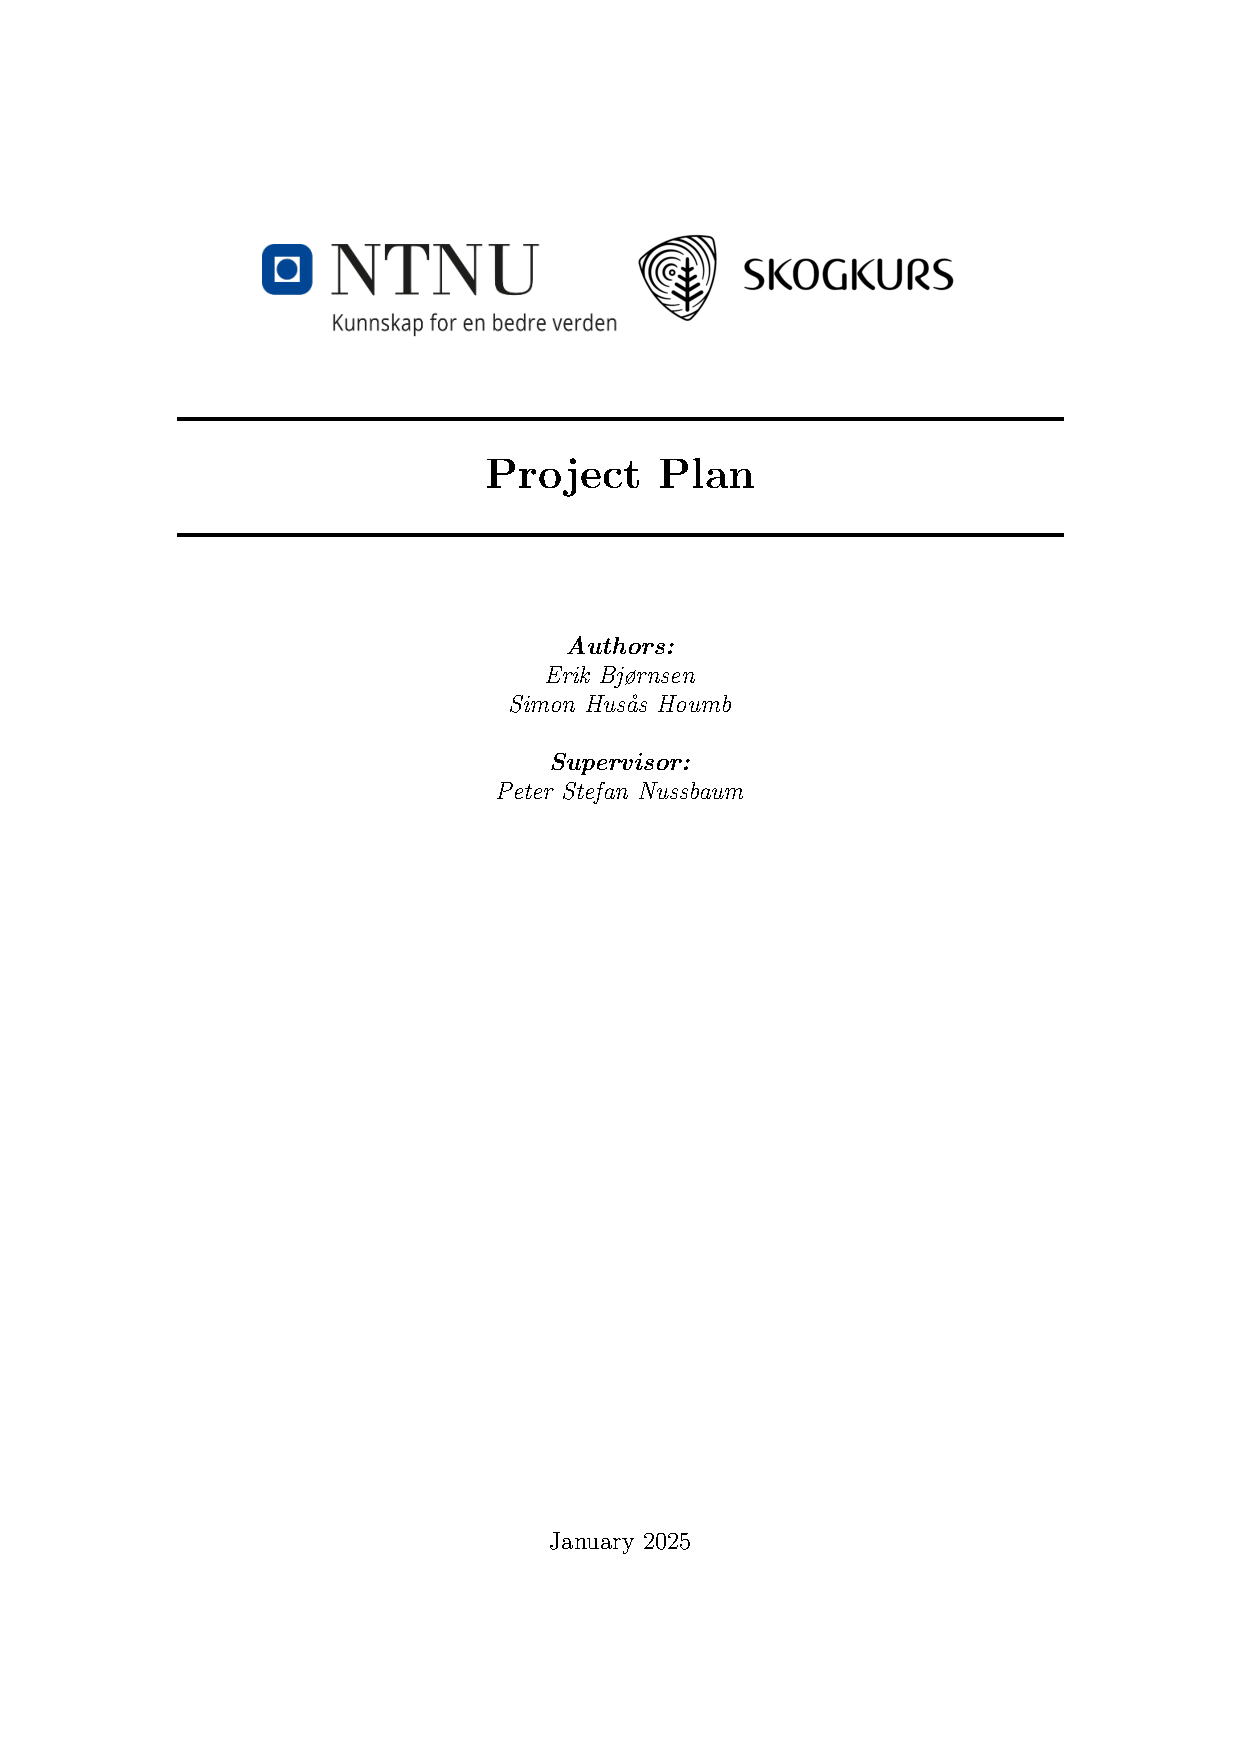
\includepdf[pages=-]{appendices/Skogkurs_Bachelor_Project_Plan_noAppendix}
\chapter{Group Contract}
\label{appendix:group_contract}
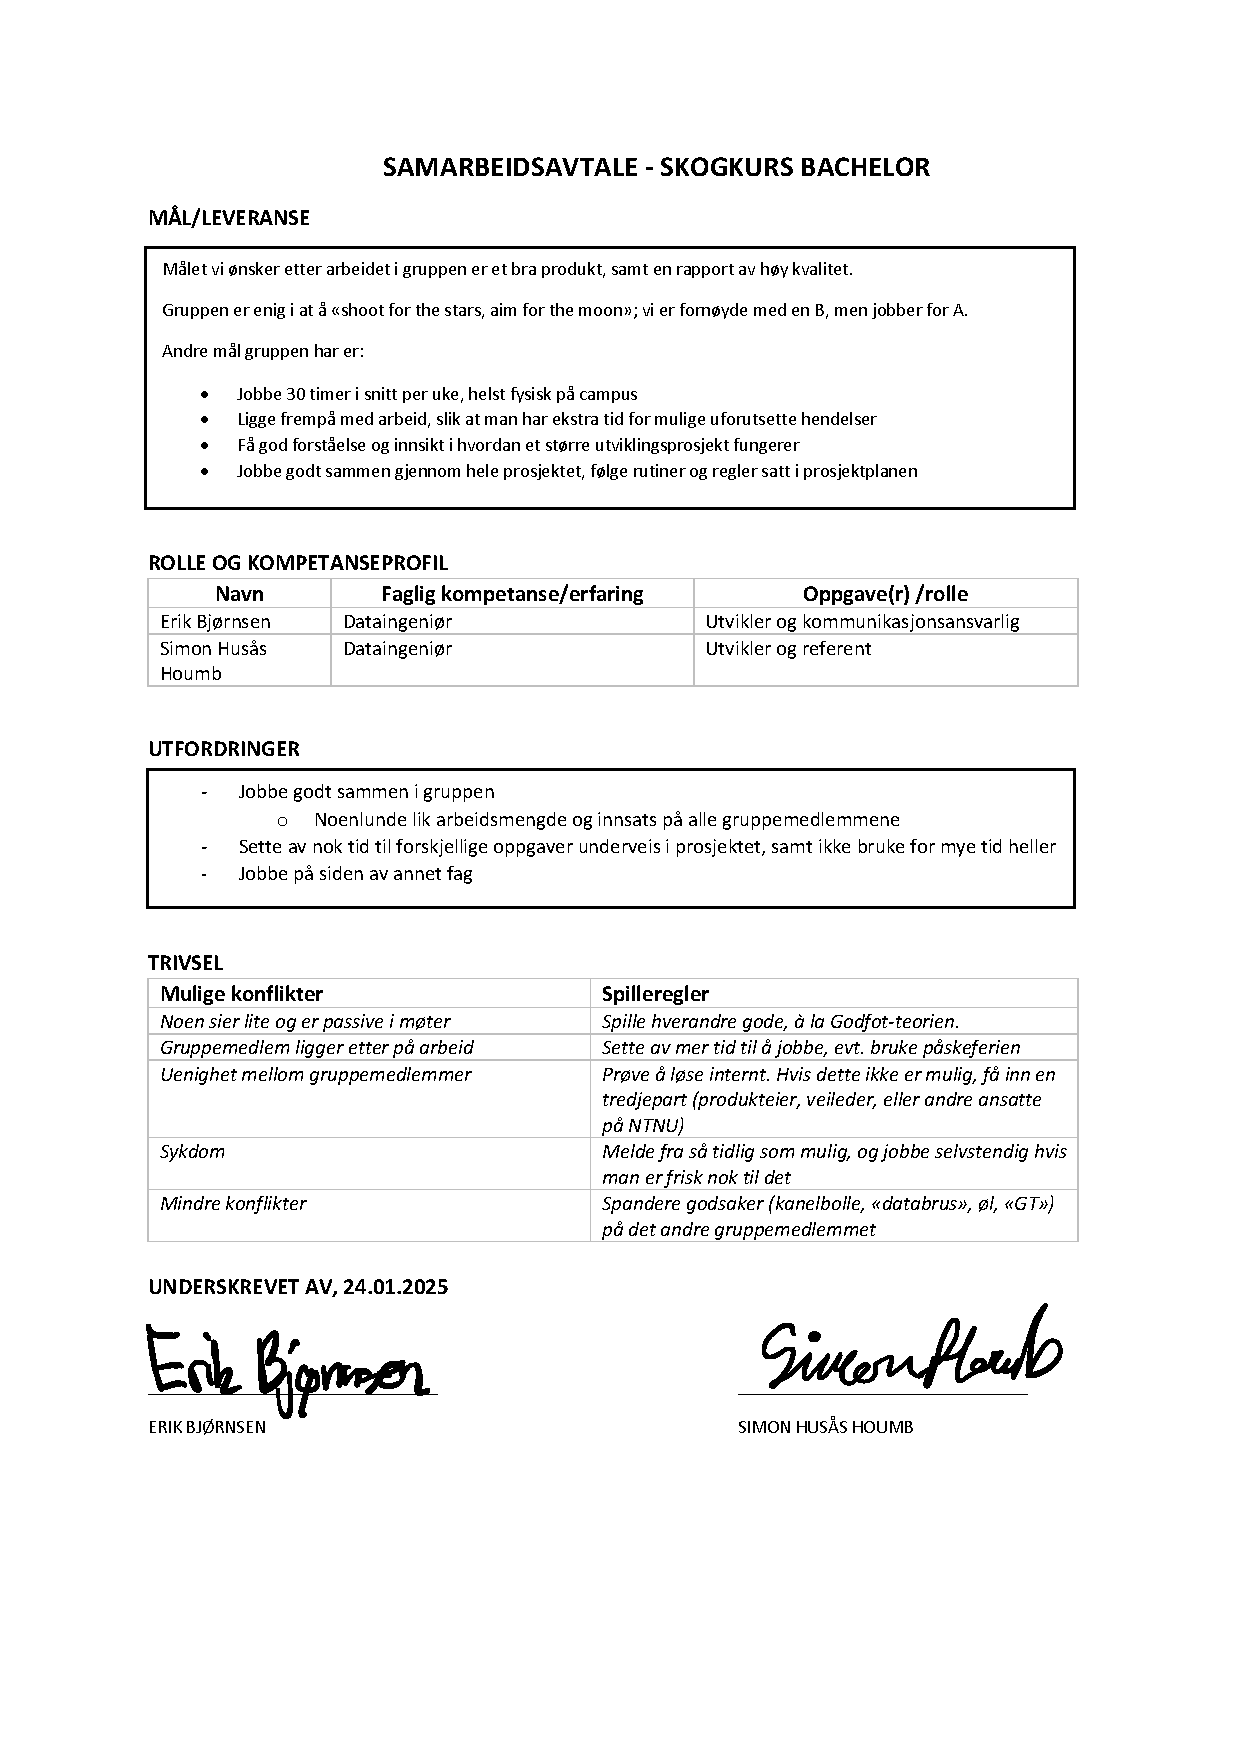
\includepdf[pages=-]{appendices/bachelor_skogkurs_samarbeidsavtale}
\chapter{Project Agreement}
\label{appendix:project_agreement}

\includepdf[pages=-]{appendices/standardavtale_skogkurs_bachelor.pdf}
\chapter{Task Description}
\label{appendix:task_description}
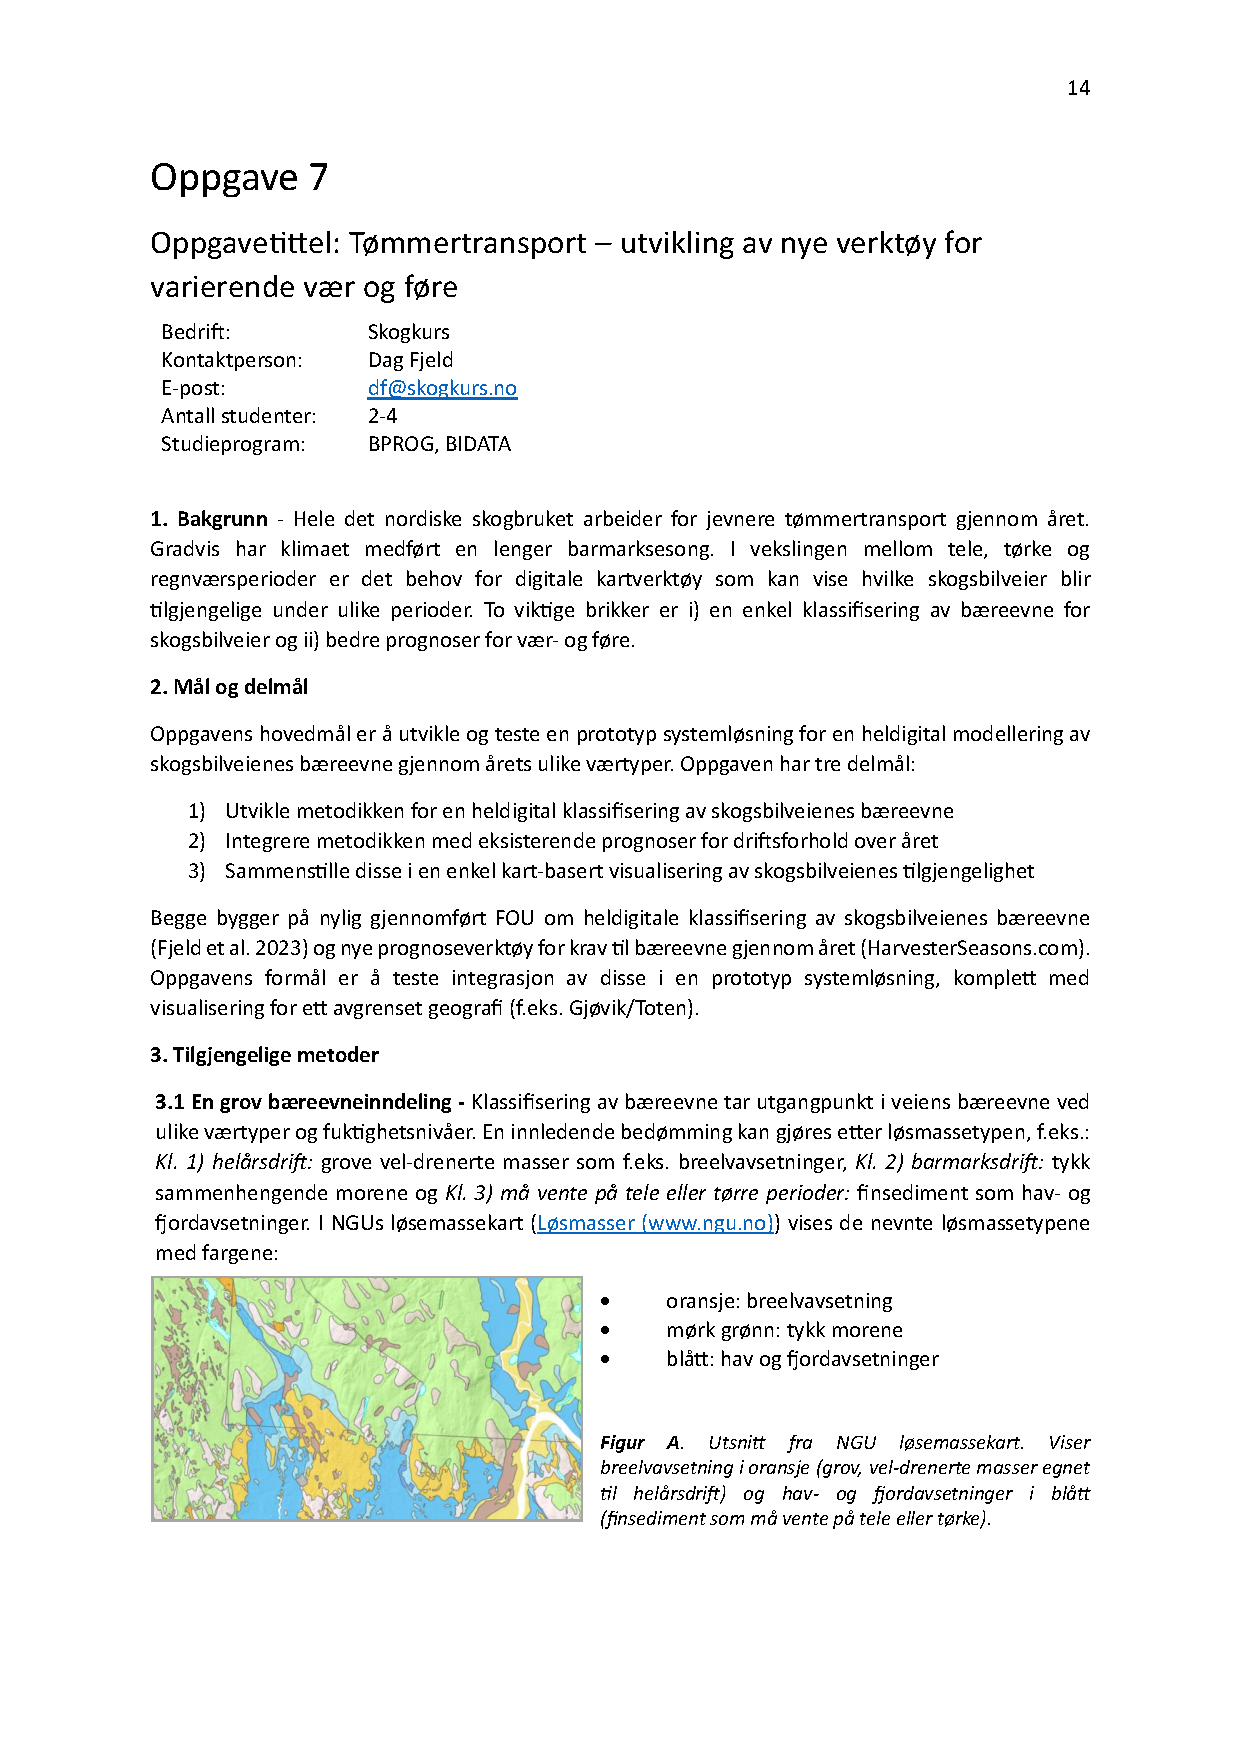
\includepdf[pages=-]{appendices/SKOGKURS_BACHELOROPPGAVE.pdf}
\chapter{Meeting Minutes}
\label{appendix:meeting_minutes}
\section*{Møte med Veileder: 2025-01-14}
\begin{itemize}
\item
  Kjernetid: 9-15, 6 timer hver dag. Vi har forelesning på mandager
  14-16 og onsdager 10-12, og gruppearbeid i samme fag som vil ta litt
  av kjernetiden første ukene.
\item
  Møte: Ukentlig med veileder, og annen hver uke med oppdragsgiver?
\item
  Ha klart spørsmål om kravspesifikasjon til Dag
\end{itemize}

\section*{Møte med Veileder og
Produkteier: 2025-01-21}

\subsection*{Agenda}
\begin{itemize}
\item
  Referere til andre sine bacheloroppgaver i prosjektplan?
\item
  Flere MVPer? Vi har nå tenkte 1 MVP midt i mars for user-testing
\item
  Få en gjennomgang til av
\item
  Annen data og utregning
\item
  NASA SMAP og ESA Sentinel-1
\item
  Hvilke data skal brukes
\item
  Hvordan få prognose frem i tid, bruke verktøy som allerede finnes
  eller lage selv?
\item
  Prosjektplan
\item
  Constraints
\item
  Delimitation (er Norge for stort område å fokusere på)
\end{itemize}

\begin{enumerate}
\item
  Dag
\item
  Kanskje Dag kan si litt om oppgaven til Peter
\item
  Gå gjennom det vi har hittil (prosjektplan, gantt)
\item
  Spørsmål
\end{enumerate}

\subsection*{Notater}
\textbf{Product \& Impact Goals:} 
\begin{itemize}
    \item Ligger på linje med Skogkurs'
forventninger
\item Impact (reduced uncertainty)
\end{itemize}
\textbf{Brukere:} 
\begin{itemize}
    \item \emph{Transportleder}
    \item Sjåfører
    \item ``Personer med kunnskap i feltet''
\end{itemize}
\textbf{Prognose:} 1-2 uker\\
\textbf{Fargekoding av vei (trafikklys):} Rød, gul, grønn\\
\textbf{Område:} Begrenset område - Gjøvik, steder det faktisk kan
bruke. For mye data.\\
\textbf{Bruk av data / variabler (begrensning):}
\begin{itemize}
    \item (Ikke konkret rett valg av data, mål å få testet at et produkt fungerer)
    \item \emph{Løsmasser}
    \item Markfuktighet
    \item Teledyp
    \item Grunnvannstilstand
    \item Skogbilveier
    \item Variere for forskjellige områder hvor det er relevant
    \item Evt. snitt data hvor flere lag brukes
    \item (ikke tenk på vekt av last)
\end{itemize}

\textbf{Brukertesting:} \\
\begin{itemize}
    \item Tidlig Wireframe slik at for teste tidlig versjon
    \item For transportledere, hjelp fra Skogkurs
\end{itemize}
\textbf{Begynne med å definere data som trengs og skal brukes i februar}
\begin{itemize}
    \item Nibio skogsportal (WMS)
    \item Traktor og skogsbilvei
    \item senorge - raster
\end{itemize}


\section*{Møte med Veileder: 2025-01-28}

\subsection*{Agenda:}
\begin{itemize}

\item
  Referere til andre sine bacheloroppgaver i prosjektplan?
\item
  Hvor spesifikt skal produktmål være?
\item
  I avsnitt om scrum, skal vi skrive om hvorfor vi ikke valgte de andre
  metodene?
\item
  Scope: burde man nevne data fra rapportene til Dag Fjeld?
\item
  Gjennomgang av scope, domain og task desc.
\end{itemize}

\subsection*{Notat:}

\begin{itemize}
\item
  Fokus på rapport, få med det som gikk bra, og hva som var utfordrende
\item
  Kartlegging i februar (data)
\item
  Finne kriteriene for data som skal eller kan brukes for å
  tilfredsstille krav
\item
  Se gjennom rapportene til D. Fjeld (abstrakt, introduksjon,
  konklusjon)

  \begin{itemize}
  \item
    Se om andre rapporter er referert
  \end{itemize}
\item
  Hvor mange uker satt av for rapport?:

  \begin{itemize}
  \item
    Kreves litt mer tid, men finn balanse
  \end{itemize}
\item
  Få teksten lest over av noen eksterne (andre studenter, familie?)

  \begin{itemize}
  \item
    Sette av litt tid for finpussing da for at noen skal lese over
  \item
    Passe på å ha en ``rød tråd'' gjennom rapporten, tenke på
    overgangene mellom deler av rapporten
  \end{itemize}
\item
  Kanskje finne lignende bachelor
\item
  Referer til andre oppgaver (ikke kopier rett fra teksten)
\item
  Skrive om SDLC

  \begin{itemize}
  \item
    Vise at man vet om andre metoder
  \item
    men ikke skrive for langt
  \item
    Finne argumenter for valg man har tatt, også andre steder i teksten
  \end{itemize}
\item
  Scope:

  \begin{itemize}
  \item
    Skogsdrift, tungtransport
  \item
    Kart
  \end{itemize}
\item
  Task description:

  \begin{itemize}
  \item
    Steg for å nå målet
  \item
    Analyse av kriterier som trengs for å nå mål
  \item
    Implementasjon av kart og webside
  \end{itemize}
\item
  Impact Goals

  \begin{itemize}
  
  \item
    Kanskje ha med noe om bærekraft, miljø, etc.
  \end{itemize}
\end{itemize}

\section*{Møte med Veileder: 2025-02-04}

\subsection*{Notat}
\begin{itemize}
\item
  Spørre produkteier om dataressurser vi har funnet
\end{itemize}

\section*{Møte med Produkteier: 2025-02-10}

\subsection*{Spørsmål}

\begin{itemize} 
\item
  OpenMeteo Ensemble API

  \begin{itemize}
  \item
    Hvor dyp jordfuktighet er nødvendig?
  \item
    Hvor nøyaktig er OpenMeteo?
  \end{itemize}
\item
  Detaljert info for skogsveg fra NIBIO: \\
  https://kilden.nibio.no/skogsbilveger\_ws/skogsbilveiInfo?sveiid=3407-14-1
\end{itemize}

\subsection*{Notat}

\begin{itemize}
\item
  Når vegen ble bygd: ØKS? Landbruksdirektoratet

  \begin{itemize}
  
  \item
    Kategorisere vegene i klasser
  \item
    Nyere og bedre veier etter 2015
  \end{itemize}
\item
  Hva er vegen bygd av
\item
  Forskjellige høydenivå på veger
\item
  Hvordan bruke soil moisture

  \begin{itemize}
  \item
    Sette klasser
  \end{itemize}
\item
  Grenser for data

  \begin{itemize}
  \item
    Kanskje ha dynamiske grenser (som kan endres av bruker)?
  \item
    Sette grenser ved bruk av historisk data?
  \end{itemize}
\item
  Ha med historisk data, da OpenMeteo kanskje ikke støtter dette.
\end{itemize}

\section*{Møte med Veileder: 2025-02-11}

\subsection*{Agenda}

\begin{itemize}
\item
  Snakke om samtalen med Dag Fjeld
\item
  Plakat/rapportmal 
\end{itemize}

\subsection*{Notat}
\begin{itemize}
    \item
      Skal spørre Pål om rapportmal
    \item
      Notere ned detaljer allerede for å ha med i den endelige rapporten
    \item
      Får mal på lynkurs, kan også finne på nett
    \item
      Info blir også gitt om plakat senere på seminar om presentasjon
\end{itemize}

\section*{Møte med Veileder: 2025-02-20}

\subsection*{Agenda}

\begin{itemize}
\item
  Vise fremgang av webside
\end{itemize}

\subsection*{Notat}

\begin{itemize}
    \item Husk å notere vanskeligheter underveis for å ha med i rapporten senere
\end{itemize}

\section*{Møte med Veileder: 2025-02-24}

\subsection*{Agenda}
\begin{itemize}
\item
  Vise fremgang av webside før møte med produkteier
\end{itemize}


\section*{Møte med Produkteier: 2025-02-25}

\subsection*{Agenda}

\begin{itemize}
\item
  Vise frem proto-prototype av webside
\end{itemize}
\subsection*{Notat}
\begin{itemize}
\item
  Copernicus, evt. prognose
\item
  Få implementert open-meteo soil moisture / soil temperature
\item
  Teledyp grenser:

  \begin{itemize}
  \item
    Både 0-7cm og 7-28cm jordtemperatur er null = grønt lys
  \item
    Jordfuktighet forskjell mellom forskjellige jordarter
  \end{itemize}
\end{itemize}

\section*{Møte med Veileder: 2025-03-04}

\subsection*{Agenda}

\begin{itemize}
\item
  Snakke om møte med produkteier forrige uke
\item
  Hva planen er fremover for denne sprinten
\end{itemize}

\subsection*{Notat}

\begin{itemize}
\item
  For klassifisering av skogsbilveg

  \begin{itemize}
  \item
    Se skiforeningens side
  \end{itemize}
\item
  Få med utfordringer, blindveier i prosessen etc. i rapport
\end{itemize}

\section*{Møte med Veileder: 2025-03-13}

\subsection*{Agenda}

\begin{itemize}
\item
  Fullt fokus på bacheloroppgaven fra nå
\end{itemize}

\subsection*{Notat}

\begin{itemize}
\item
  Se rapportskrivings krasjkurs
\item
  Rapportskrivingskurs 27. Mars
\item
  Første utkast av rapport til påske f.eks. tirsdag 8. april, gi til
  veileder for tilbakemelding
\item
  Tilbakemelding på utkast etter påske tirsdag 22. april
\end{itemize}

\section*{Møte med Veileder: 2025-03-18}

\subsection*{Agenda}
\begin{itemize}
\item
  Forside til rapporten, skal vi ha med egen eller blir den generert ved
  innlevering
\item
  Eksempler på ``A''-rapporter
\item
  Hva burde være med av kapitler, særlig introduksjon. F.eks. skal ikke
  ha med gruppebakgrunn eller noe personlig om gruppen (ifølge Hjelmås)
\item
  Mellomrom eller innrykk mellom avsnitt
\item
  Referanse har tomt parantes hvis man ikke legger til dato for når
  siden ble sist oppdatert. Er dette nødvendig og hvis det ikke er
  oppgitt kan man bruke ``n.d.'' (no date)
\item
  Chapter vs.~Section. Virker litt unaturlig at det står Chapter 1, 2, 3
  osv.
\item
  Latex tar med forfatter og tittel på hver partall side, f.eks.
  ``erbj\&simonhou@NTNU: Lumber transport'' er dette meningen?
\item
  Er det relevant å ta med som utfordring at tidsfordeling med et annet
  fag på siden av bachelor
\end{itemize}
  
\subsection*{Notat}
\begin{itemize}
\item
  Kan ta med i rapporten at man finner frem til løsninger ved å sparre
  med AI.
\item
  Forside til rapporten, skal vi ha med egen eller blir den generert ved
  innlevering

  \begin{itemize}
  \item
    \emph{Får svar før innlevering.}
  \end{itemize}
\item
  Eksempler på ``A''-rapporter

  \begin{itemize}
  \item
  \end{itemize}
\item
  Hva burde være med av kapitler, særlig introduksjon. F.eks. skal ikke
  ha med gruppebakgrunn eller noe personlig om gruppen (ifølge Hjelmås)

  \begin{itemize}
  \item
    \emph{Hvis man skal ta det med så hold det kort.}
  \item
    \emph{Er mulig å få A selv om man tar med.}
  \end{itemize}
\item
  Mellomrom eller innrykk mellom avsnitt

  \begin{itemize}
  \item
    \emph{Mellomrom}
  \end{itemize}
\item
  Referanse har tomt parentes hvis man ikke legger til dato for når
  siden ble sist oppdatert. Er dette nødvendig og hvis det ikke er
  oppgitt kan man bruke ``n.d.'' (no date)?

  \begin{itemize}
  
  \item
    \emph{Prøv å fjern parentesen hvis ingen dato er oppgitt istedenfor
    å bruke n.d. eller no date}
  \end{itemize}
\item
  Chapter vs.~Section. Virker litt unaturlig at det står Chapter 1, 2, 3
  osv.

  \begin{itemize}
  
  \item
    \emph{Ja, chapter skal ytterst}
  \end{itemize}
\item
  Latex tar med forfatter og tittel på hver partall side, f.eks.
  ``erbj\&simonhou@NTNU: Lumber transport'' er dette meningen?

  \begin{itemize}
  
  \item
    \emph{At kapittel står er fint, men må ikke ha med forfatter
    og/eller tittel.}
  \end{itemize}
\item
  Er det relevant å ta med som utfordring at tidsfordeling med et annet
  fag på siden av bachelor. Også med tidsfordeling om at vi kun er 2 i
  gruppen.

  \begin{itemize}
  
  \item
    \emph{Hvis man kan ta med på en bra måt så ta med på en objektiv
    måte, ikke for spesifikt.}
  \item
    \emph{Ikke nevn følelser (adjektiver), ikke spesifiser 2 i gruppen
    (sensor vet det). Heller nevn at man var litt for optimistisk på
    tiden man hadde.}
  \item
    \emph{Trenger kanskje ikke nevne hvis det ikke ble lovet i planen
    eller at det ikke var et krav fra produkteier.}
  \end{itemize}
\item
  Ha tekst for hvert nye kapittel (som forklarer innholdet for
  kapitellet). Hvis man er i et senere kapittelet kan denne setningen
  gjerne inneholde et slags\\
\item
  Vær flink til å ha med figurer for å forklare prinsipper eller hvordan
  produktet fungerer, samt selve prossesen av prosjektet.

  \begin{itemize}
  \item
    Figurer er også fint å bruke i presentasjonen
  \end{itemize}
\item
  Universell Utforming burde tas med, f.eks. ha med spørsmål på
  brukertesting.

  \begin{itemize}
  \item
    Hvis man ikke finner en perfekt løsning for f.eks. design, så nevn
    det i rapport uansett. Eks. fargeblindhet
  \end{itemize}
\end{itemize}
\chapter{Use Case Specifications}
\label{appendix:use_case_specifications}

\begin{table}[h]
    \centering
    \renewcommand{\arraystretch}{1.5}
    \begin{tabularx}{\textwidth}{|l|X|}
        \hline
        \rowcolor{gray!20}
        \textbf{Use Case Name} & Toggle Map Layer \\
        \hline
        \textbf{Actor(s)} & User \\
        \hline
        \textbf{Description} & The user can toggle specific map layers to control the visibility of different map layers. This functionality allows users to select from various map layers. The selected layer is then displayed, and relevant information is shown in the map legend sidebar. \\
        \hline
        \textbf{Priority} & High \\
        \hline
        \textbf{Pre-Condition(s)} & The user must have a stable internet connection and the website open. The website and server and map server must be deployed and running.\\
        \hline
        \textbf{Post-Condition(s)} & The map will be updated with the specific map layer that was toggled. The map legend will also be visible in the legend sidebar. \\
        \hline
        \textbf{Basic Path} &  
        \begin{enumerate}[label=,left=0pt]
            \item 1. User presses the map layer ("kartlag") button to open the map layer sidebar.
            \item 2. User clicks the toggle button for the specific map layer to toggle.
            \item 3. The system updates the map with the selected layer.
        \end{enumerate} \\
        \hline
        \textbf{Exception Path} & 
        \begin{enumerate}[label=,left=0pt]
            \item 0. User does not have a stable internet connection and can not connect to the website.
            \item 2a. Either the backend server or the map server is not responding, and no map data is received.
        \end{enumerate} \\
        \hline
    \end{tabularx}
    \caption[Use Case Specification: Toggle Map Layer]{Use case for toggling a map layer.}
    \label{tab:use_case_toggle_layer_appendix}
\end{table}

\begin{table}[h]
    \centering
    \renewcommand{\arraystretch}{1.5}
    \begin{tabularx}{\textwidth}{|l|X|}
        \hline
        \rowcolor{gray!20}
        \textbf{Use Case Name} & Show Map Legend \\
        \hline
        \textbf{Actor(s)} & User \\
        \hline
        \textbf{Description} & The user can show legends for the map layers that are toggled on. \\
        \hline
        \textbf{Priority} & Medium \\
        \hline
        \textbf{Pre-Condition(s)} & The user must have a stable internet connection and the website open. The website and server and map server must be deployed and running. The map layer for the specific legend must be toggled before the legend is visible. \\
        \hline
        \textbf{Post-Condition(s)} & The legend sidebar will contain the legend for the toggled map layers. If no map layer is toggled, it will be empty. \\
        \hline
        \textbf{Basic Path} &  
        \begin{enumerate}[label=,left=0pt]
            \item 1. User presses the map layer ("kartlag") button to open the map layer sidebar.
            \item 2. User clicks the toggle button for the specific map layer to toggle.
            \item 3. The system updates the map with the selected layer.
            \item 4. User presses the map legend ("tegnforklaring") button to open the legend sidebar showing all the legends for the toggled map layers.
        \end{enumerate} \\
        \hline
        \textbf{Alternative Path} & 
        \begin{enumerate}[label=,left=0pt]
            \item 1. User presses the map legend ("tegnforklaring") button to open the legend sidebar.
            \item 2. User presses the map layer ("kartlag") button to open the map layer sidebar.
            \item 3. User clicks the toggle button for the specific map layer to toggle.
            \item 4. The opened legend sidebar is updated with the legend for the toggled map layer.
        \end{enumerate} \\
        \hline
        \textbf{Exception Path} & 
        \begin{enumerate}[label=,left=0pt]
            \item 0. User does not have a stable internet connection.
            \item 1. Either the backend server or the map server is not responding, and no map data is received.
            \item 2. No / The incorrect map layer is toggled.
        \end{enumerate} \\
        \hline
    \end{tabularx}
    \caption[Use Case Specification: Show Map Legend]{Use case for showing the map legends.}
    \label{tab:use_case_show_legend_appendix}
\end{table}

\begin{table}[h]
    \centering
    \renewcommand{\arraystretch}{1.5}
    \begin{tabularx}{\textwidth}{|l|X|}
        \hline
        \rowcolor{gray!20}
        \textbf{Use Case Name} & Center on User Location \\
        \hline
        \textbf{Actor(s)} & User \\
        \hline
        \textbf{Description} & The user can center the map on their current location. The system requires permission from the user to access their location. \\
        \hline
        \textbf{Priority} & Medium \\
        \hline
        \textbf{Pre-Condition(s)} & The user must have a stable internet connection and the website open. The server and map server must be deployed and running. \\
        \hline
        \textbf{Post-Condition(s)} & The map view will center on the user's current location. If permission is denied, the map will not center on their location. \\
        \hline
        \textbf{Basic Path} &  
        \begin{enumerate}[label=,left=0pt]
            \item 1. User clicks the "Center on User Location" button.
            \item 2. System requests permission to access the user's location.
            \item 3. User grants permission.
            \item 4. System retrieves the user's current location and centers the map on it.
        \end{enumerate} \\
        \hline
        \textbf{Alternative Path} & 
        \begin{enumerate}[label=,left=0pt]
            \item 1. User clicks the "Center on User Location" button.
            \item 2. The user has already granted permission.
            \item 3. System retrieves the user's current location and centers the map on it.
        \end{enumerate} \\
        \hline
        \textbf{Exception Path} & 
        \begin{enumerate}[label=,left=0pt]
            \item 0. User does not have a stable internet connection.
            \item 1. The user does not grant permission to share location.
        \end{enumerate} \\
        \hline
    \end{tabularx}
    \caption[Use Case Specification: Center on User Location]{Use case for centering on the user's location.}
    \label{tab:use_case_center_location_appendix}
\end{table}


\begin{table}[h]
    \centering
    \renewcommand{\arraystretch}{1.5}
    \begin{tabularx}{\textwidth}{|l|X|}
        \hline
        \rowcolor{gray!20}
        \textbf{Use Case Name} & Zoom In/Out \\
        \hline
        \textbf{Actor(s)} & User \\
        \hline
        \textbf{Description} & The user can zoom in or out on the map, which will in turn update the map accordingly. \\
        \hline
        \textbf{Priority} & High \\
        \hline
        \textbf{Pre-Condition(s)} & The user must have a stable internet connection and the website open. The server and map server must be deployed and running. \\
        \hline
        \textbf{Post-Condition(s)} & The map will be zoomed in or out. \\
        \hline
        \textbf{Basic Path} &  
        \begin{enumerate}[label=,left=0pt]
            \item 1. User clicks the zoom in or zoom out button.
            \item 2. The map updates to reflect the new zoom level.
        \end{enumerate} \\
        \hline
        \textbf{Alternative Path} & 
        \begin{enumerate}[label=,left=0pt]
            \item 1. User zooms in or out using the scroll wheel.
            \item 2. The map updates accordingly.
        \end{enumerate} \\
        \hline
        \textbf{Exception Path} & 
        \begin{enumerate}[label=,left=0pt]
            \item 0. User does not have a stable internet connection.
            \item 1. The user attempts to zoom beyond the allowed range.
            \item 2. The system restricts further zooming and maintains the current zoom level.
        \end{enumerate} \\
        \hline
    \end{tabularx}
    \caption[Use Case Specification: Zoom In/Out]{Use case for zooming in/out on map.}
    \label{tab:use_case_zoom_appendix}
\end{table}

\begin{table}[h]
    \centering
    \renewcommand{\arraystretch}{1.5}
    \begin{tabularx}{\textwidth}{|l|X|}
        \hline
        \rowcolor{gray!20}
        \textbf{Use Case Name} & Pan/Drag Map \\
        \hline
        \textbf{Actor(s)} & User \\
        \hline
        \textbf{Description} & The user interacts with the map by clicking and dragging to move the view in different directions, allowing them to navigate to different areas. \\ 
        \hline
        \textbf{Priority} & High \\
        \hline
        \textbf{Pre-Condition(s)} & The user must have a stable internet connection and the website open. The server and map server must be deployed and running. The user is using a device that supports click-and-drag or touch gestures.\\
        \hline
        \textbf{Post-Condition(s)} & The map view updates to reflect the user's movement. If the user reaches the map boundaries, further panning is restricted. \\
        \hline
        \textbf{Basic Path} &  
        \begin{enumerate}[label=,left=0pt]
            \item 1. The user clicks and holds the left mouse button (or touches the screen on a touch device).
            \item 2. The user drags the cursor (or moves their finger) to pan the map.
            \item 3. The map moves in the corresponding direction.
        \end{enumerate} \\
        \hline
        \textbf{Exception Path} & 
        \begin{enumerate}[label=,left=0pt]
            \item 0. User does not have a stable internet connection.
            \item 1. The user tries to pan beyond the available map boundaries.
            \item 2. The system prevents further movement in that direction.
        \end{enumerate} \\
        \hline
    \end{tabularx}
    \caption[Use Case Specification: Pan/Drag Map]{Use case for panning/dragging map.}
    \label{tab:use_case_drag_map_appendix}
\end{table}

\begin{table}[h]
    \centering
    \renewcommand{\arraystretch}{1.5}
    \begin{tabularx}{\textwidth}{|l|X|}
        \hline
        \rowcolor{gray!20}
        \textbf{Use Case Name} & Adjust Map Layer Opacity \\
        \hline
        \textbf{Actor(s)} & User \\
        \hline
        \textbf{Description} & The user adjusts the opacity of a selected map layer to control its visibility, allowing better comparison with other layers or the base map. \\\hline
        \textbf{Priority} & Low \\
        \hline
        \textbf{Pre-Condition(s)} & The user must have a stable internet connection and the website open. The server and map server must be deployed and running. The specific map layer must be toggled on for opacity adjustments to be visible. \\
        \hline
        \textbf{Post-Condition(s)} & The selected map layer’s opacity is updated in real time. The visual representation of the layer changes on the map. \\
        \hline
        \textbf{Basic Path} &  
        \begin{enumerate}[label=,left=0pt]
            \item 1. User presses the map layer ("kartlag") button to open the map layer sidebar.
            \item 2. User clicks the toggle button for the specific map layer to toggle.
            \item 3. The system updates the map with the selected layer.
            \item 4. The user adjusts the opacity using the opacity slider.
            \item 5. The system updates the opacity of the selected map layer in real time. 
        \end{enumerate} \\
        \hline
        \textbf{Exception Path} & 
        \begin{enumerate}[label=,left=0pt]
            \item 0. User does not have a stable internet connection.
            \item 1. The map layer is not toggled and the opacity change is not visible.
        \end{enumerate} \\
        \hline
    \end{tabularx}
    \caption[Use Case Specification: Adjust Map Layer Opacity]{Use case for changing map opacity.}
    \label{tab:use_case_map_opacity_appendix}
\end{table}

\begin{table}[h]
    \centering
    \renewcommand{\arraystretch}{1.5}
    \begin{tabularx}{\textwidth}{|l|X|}
        \hline
        \rowcolor{gray!20}
        \textbf{Use Case Name} & Query a Map Layer \\
        \hline
        \textbf{Actor(s)} & User \\
        \hline
        \textbf{Description} & The user queries a specific map layer to retrieve detailed information about a selected feature. This allows the user to interact with and understand the data represented on the map. \\        \hline
        \textbf{Priority} & Medium \\
        \hline
        \textbf{Pre-Condition(s)} & The user must have a stable internet connection and the website open. The server and map server must be deployed and running. The specific map layer must be toggled on for opacity adjustments to be visible. \\
        \hline
        \textbf{Post-Condition(s)} & Information about the selected feature is displayed to the user. \\
        \hline
        \textbf{Basic Path} &  
        \begin{enumerate}[label=,left=0pt]
            \item 1. The user clicks on a feature within an active map layer.
            \item 2. The system queries the relevant data associated with the feature.
            \item 3. The system displays the retrieved information in a popup or sidebar.
        \end{enumerate} \\
        \hline
        \textbf{Alternative Path} & 
        \begin{enumerate}[label=,left=0pt]
            \item 1. The user selects a different feature, triggering a new query.
        \end{enumerate} \\
        \hline
        \textbf{Exception Path} & 
        \begin{enumerate}[label=,left=0pt]
            \item 0. User does not have a stable internet connection.
            \item 1. No map layer is toggled on.
            \item 2. The selected feature does not contain queryable data.
        \end{enumerate} \\
        \hline
    \end{tabularx}
    \caption[Use Case Specification: Query a Map Layer]{Use case for querying a map layer.}
    \label{tab:use_case_query_map_appendix}
\end{table}

\begin{table}[h]
    \centering
    \renewcommand{\arraystretch}{1.5}
    \begin{tabularx}{\textwidth}{|l|X|}
        \hline
        \rowcolor{gray!20}
        \textbf{Use Case Name} & Select Map Date \\
        \hline
        \textbf{Actor(s)} & User \\
        \hline
        \textbf{Description} & The user selects a date to view map data from a specific time period. This allows the user to look at either historical data or a forecast. \\
        \hline
        \textbf{Priority} & High \\
        \hline
        \textbf{Pre-Condition(s)} & The user must have a stable internet connection and the website open. The server and map server must be deployed and running. Time-based map data must be available for selected map layer. \\
        \hline
        \textbf{Post-Condition(s)} & The map updates to display data corresponding to the selected date. \\
        \hline
        \textbf{Basic Path} &  
        \begin{enumerate}[label=,left=0pt]
            \item 1. The user opens the date selection menu.
            \item 2. The user selects a specific date.
            \item 3. The system loads the corresponding map data.
            \item 4. The map updates to reflect the chosen date.
        \end{enumerate} \\
        \hline
        \textbf{Alternative Path} & 
        \begin{enumerate}[label=,left=0pt]
            \item 1. The user changed the date by using the next/previous day, week, or year buttons.
            \item 2. The system loads the corresponding map data.
            \item 3. The map updates to reflect the chosen date.
        \end{enumerate} \\
        \hline
        \textbf{Exception Path} & 
        \begin{enumerate}[label=,left=0pt]
            \item 0. User does not have a stable internet connection.
            \item 1. No map layer is active.
            \item 2a. The active map layer does not support the selected date.
            \item 2b. The map is not shown for that selected date.
            \item 3a. A invalid date is selected.
            \item 3b. The date does not change to the invalid date.
        \end{enumerate} \\
        \hline
    \end{tabularx}
    \caption[Use Case Specification: Select Map Date]{Use case for selecting the date of the map.}
    \label{tab:use_case_date_map_appendix}
\end{table}

\begin{table}[h]
    \centering
    \renewcommand{\arraystretch}{1.5}
    \begin{tabularx}{\textwidth}{|l|X|}
        \hline
        \rowcolor{gray!20}
        \textbf{Use Case Name} & Change Base Map Layer \\
        \hline
        \textbf{Actor(s)} & User \\
        \hline
        \textbf{Description} & The user changes the base map layer to adjust the visual presentation of the map. This allows switching between terrain maps, or street maps for better context. \\
        \hline
        \textbf{Priority} & Low \\
        \hline
        \textbf{Pre-Condition(s)} & The user must have a stable internet connection and the website open. The server and map server must be deployed and running. \\
        \hline
        \textbf{Post-Condition(s)} & The map updates to display the selected base layer. \\
        \hline
        \textbf{Basic Path} &  
        \begin{enumerate}[label=,left=0pt]
            \item 1. The user presses the button to change to the selected base layer.
            \item 2. The system loads and applies the new base map layer.
        \end{enumerate} \\
        \hline
        \textbf{Exception Path} & 
        \begin{enumerate}[label=,left=0pt]
            \item 0. User does not have a stable internet connection.
        \end{enumerate} \\
        \hline
    \end{tabularx}
    \caption[Use Case Specification: Change Base Map Layer]{Use case for changing the base layer of the map.}
    \label{tab:use_case_base_layer_appendix}
\end{table}
\chapter{Superficial Deposits Code Values}
\label{appendix:superficial_deposit_codes}
\begin{longtable}{|p{3.5cm}|p{6.2cm}|c|}
    \hline
    \textbf{Navn} & \textbf{Beskrivelse} & \textbf{Kodeverdi}\\ 
    \endfirsthead
    
    \hline
    \textbf{Navn} & \textbf{Beskrivelse} & \textbf{Kodeverdi}\\ 
    \endhead
    \hline
    
    Løsmasser / berggrunn under vann, uspesifisert & Brukes for en avsetning der genetisk opprinnelse ikke er påvist, og det er heller ikke bestemt  om sedimentet er av marin opprinnelse. & 1 \\ \hline
    Morenemateriale, uspesifisert & Materiale plukket opp, transportert og avsatt av isbreer. Det er vanligvis, dårlig sortert og kan inneholde alt fra leir til stein og blokk. Mektighet, morenetype og overflateform kan variere. Benyttes ved kartframstilling i svært små målestokker. & 10 \\ \hline
    Morenemateriale, sammenhengende dekke, stedvis med stor mektighet & Materiale plukket opp, transportert og avsatt av isbreer, vanligvis hardt sammenpakket, dårlig sortert og kan inneholde alt fra leir til stein og blokk. Moreneavsetninger med tykkelse fra 0,5 m til flere ti-talls meter. Det er få eller ingen fjellblotninger i området. & 11 \\ \hline
    Morenemateriale, usammenhengende eller tynt dekke over berggrunnen & Materiale plukket opp, transportert og avsatt av isbreer. Det er vanligvis hardt sammenpakket, dårlig sortert og kan inneholde alt fra leir til stein og blokk. Områder med grunnlendte moreneavsetninger/hyppige fjellblotninger. Tykkelsen på avsetningene er normalt mindre enn 0,5 m, men den kan helt lokalt være noe mer. & 12 \\ \hline
    Moreneleire & Morenemateriale med særlig høyt leir- og siltinnhold, oftest meget kompakt. & 13 \\ \hline
    Avsmeltningsmorene (Ablasjonsmorene) & Hauger og rygger med løst lagret, delvis vannbehandlet og noe sortert morenemateriale avsatt fra stagnerende breer (dødis). Terrenget er preget av haug- og ryggformer med vekslende orientering. & 14 \\ \hline
    Randmorene / randmorenebelte & Rygger eller belter av morenemateriale som er skjøvet opp foran brefronten. Materialet er usortert og inneholder alle kornstørrelser fra leir til blokk. Noen steder kan morenematerialet finnes i veksling med breelvmateriale. & 15 \\ \hline
    Drumlin & Langstrakt, rettlinjet morenerygg dannet langs isbevegelsesretningen i bunnen av en bre. Ofte stor tykkelse, avrundet form og lengden kan være opp til noen km. & 16 \\ \hline
    Rogenmorene & Rygger av morenemateriale, orientert på tvers av brebevegelsen. & 17 \\ \hline
    Breelvavsetning (Glasifluvial avsetning) & Materiale transportert og avsatt av breelver. Sedimentet består av sorterte, ofte skråstilte lag av forskjellig kornstørrelse fra fin sand til stein og blokk. Breelvavsetninger har ofte klare overflateformer som terrasser, rygger og vifter. Mektigheten er ofte flere ti-talls meter. & 20 \\ \hline
    Breelv- og elveavsetning & Materiale transportert og avsatt av elver eller breelver. Sedimentet består av sorterte lag av forskjellig kornstørrelse fra fin sand til grus og stein. Det er ikke skilt mellom breelv- og elveavsetninger. Brukes kun i spesielle tilfeller. & 21 \\ \hline
    Ryggformet breelvavsetning (Esker) & Sortert og lagdelt materiale, vesentlig sand og grus, avsatt i tunneler eller sprekker i breen. Der avsetningen er stor nok til å danne figur på kartet brukes fargen for breelvavsetninger til å angi utbredelsen og eskersymbolet til å angi ryggformen. & 22 \\ \hline
    Haugformet breelvavsetning (Kame) & Materiale avsatt av smeltevann i hulrom i breen. Store avsetninger gis fargen for breelvavsetninger i kombinasjon med symbol for kame. & 23 \\ \hline
    Bresjø-/eller brekammeravsetning (Glasilakustrin avsetning) & Finkornig materiale avsatt i bresjø eller vannfylt brekammer hvor tykkelsen er mer enn 0,5 m og arealdekningen er stor nok til å danne figur på kartet. Mektigheten kan være flere ti-talls meter. & 30 \\ \hline
    Breelv- og bresjø-/brekammeravsetning (Glasifluvial og glasilakustrin avsetning) & Materiale avsatt av breelv eller i bredemte sjøer/brekammer. Det er ikke skilt mellom breelv- og bresjø-/kammeravsetninger. & 31 \\ \hline
    Innsjøavsetning (Lakustrin avsetning) & Materiale avsatt i innsjøer hvor tykkelsen er mer enn 0,5 m. & 35 \\ \hline
    Bresjø-/brekammer og innsjøavsetning (Glasilakustrin og lakustrin avsetning) & Benyttes hvis en ønsker å slå sammen de to avsetningstypene. I tilfelle brukes ikke separate farger for bresjø og innsjø på det samme kartbladet. & 36 \\ \hline
    Strandavsetning, innsjø og/eller bresjø & Strandvaskede sedimenter med mektighet større enn 0,5 m, dannet ved bølgeaktivitet i ferskvann. Materialet er ofte rundet og godt sortert. Kornstørrelsen varierer, men sand og grus er vanligst. & 37 \\ \hline
    Hav- og fjordavsetning, uspesifisert & Benyttes ved kartframstilling i svært små målestokker der en ikke skiller etter mektighet. & 40 \\ \hline
    Hav- og fjordavsetning, sammenhengende dekke, ofte med stor mektighet & Finkornige, marine avsetninger med mektighet fra 0,5 m til flere ti-tall meter. Avsetningstypen omfatter også skredmasser fra kvikkleireskred, ofte angitt med tilleggssymbol. Det er få eller ingen fjellblotninger i området. & 41 \\ \hline
    Marin strandavsetning, sammenhengende dekke & Marine strandvaskede sedimenter med mektighet større enn 0,5 m, dannet av bølge- og strømaktivitet i strandsonen, stedvis som strandvoller. Materialet er ofte rundet og godt sortert. Kornstørrelsen varierer fra sand til blokk, men sand og grus er vanligst. Strandavsetninger ligger som et forholdsvis tynt dekke over berggrunn eller andre sedimenter. & 42 \\ \hline
    Hav- og fjordavsetning  og strandavsetning, usammenhengende eller tynt dekke over berggrunnen & Grunnlendte områder/hyppige fjellblotninger. Tykkelsen på avsetningene er normalt mindre enn 0,5 m, men den kan helt lokalt være noe større. Det er ikke skilt mellom hav-, fjord- og strandavsetning. Kornstørrelser angis normalt ikke, men kan være alt fra leir til blokk. & 43 \\ \hline
    Skjellsand & Avsetning som i stor grad består av knuste skall av kalkutskillende organismer. Er en type av bioklastisk materiale. Kornstørrelse varierer fra nesten hele skall til sand. Det kan være ansamlet store mengder av skjellsand i umiddelbar nærhet av gode skjellvekstområder. & 44 \\ \hline
    Marin gytje & Avsetning som består av finkornig materiale, silt og leir med høyt organisk innhold. Det organiske materialet er primærprodusert i vannmassene. Marin gytje finnes i områder hvor det er liten materialtransport fra land. Brukes sjelden. & 45 \\ \hline
    Elve- og bekkeavsetning (Fluvial avsetning) & Materiale som er transportert og avsatt av elver og bekker. De mest typiske formene er elvesletter, terrasser og vifter. Sand og grus dominerer, og materialet er sortert og rundet. Mektigheten varierer fra 0,5 til mer enn 10 m. & 50 \\ \hline
    Elveavsetning, sammenhengende dekke & Materiale som er transportert og avsatt av elver og bekker. De mest typiske formene er elvesletter, terrasser og vifter. Sand og grus dominerer, og materialet er sortert og rundet. Brukes kun i spesielle tilfeller. & 51 \\ \hline
    Elveavsetning, usammenhengende/tynt dekke & Grunnlendte områder med elveavsetninger. Brukes kun i spesielle tilfeller. & 52 \\ \hline
    Flomavsetning (uspesifisert) & Brukes for spesielle sedimenter avsatt ved plutselig uttapning av bresjøer. & 53 \\ \hline
    Flomavsetning, sammenhengende & Brukes for spesielle sedimenter avsatt ved plutselig uttapning av bresjøer. & 54 \\ \hline
    Flomavsetning, usammenhengende/tynt & Brukes for spesielle sedimenter avsatt ved plutselig uttapning av bresjøer. Tykkelse mindre enn 0,5 m. & 55 \\ \hline
    Vindavsetning (Eolisk avsetning) & Flygesand med tykkelse mer enn 0,5 m. & 60 \\ \hline
    Forvitringsmateriale, ikke inndelt etter mektighet & Løsmasser dannet på stedet ved fysisk eller kjemisk nedbryting av berggrunnen. Gradvis overgang til underliggende fast fjell. Brukes når en ikke skiller mellom sammenhengende og usammenhengende dekke av denne avsetningstypen. & 70 \\ \hline
    Forvitringsmateriale, sammenhengende dekke & Løsmasser dannet på stedet ved fysisk eller kjemisk nedbryting av berggrunnen. Tykkelsen er mer enn 0,5 m. & 71 \\ \hline
    Forvitringsmateriale, usammenhengende eller tynt dekke over berggrunnen & Løsmasser dannet på stedet ved fysisk eller kjemisk nedbryting av berggrunnen. Grunnlendt område med tallrike fjellblotninger. & 72 \\ \hline
    Forvitringsmateriale, stein- og blokkrikt, dannet ved frostsprengning & Blokkhav, oftest i fjellområder. & 73 \\ \hline
    Skredmateriale, ikke inndelt etter mektighet & Avsetninger dannet ved steinsprang, fjellskred, snø- eller løsmasseskred fra bratte dalsider. Uspesifisert tykkelse. & 80 \\ \hline
    Skredmateriale, sammenhengende dekke, stedvis med stor mektighet & Avsetninger dannet ved steinsprang, fjellskred, snøskred eller løsmasseskred fra bratte dalsider. Symbol viser dominerende skredtype. Tykkelsen er mer enn 0,5 m og det er få fjellblotninger i området. & 81 \\ \hline
    Skredmateriale, usammenhengende eller tynt dekke over berggrunnen & Grunnlendte områder med avsetninger fra steinsprang, fjellskred, snø- og løsmasseskred fra bratte dalsider. Symbol viser dominerende skredtype. Tykkelse mindre enn 0,5 m. & 82 \\ \hline
    Steinbreavsetning & Steinur som inneholder/har inneholdt is og derfor er i bevegelse/har vært i bevegelse som en vanlig bre. Avsetningstypen dannes under permafrostforhold. & 88 \\ \hline
    Torv og myr (Organisk materiale) & Organisk jord dannet av døde planterester, med mektigheter større enn 0,5 m. Det skilles ikke mellom ulike torvtyper. & 90 \\ \hline
    Humusdekke/tynt torvdekke over berggrunn & Områder hvor humusdekket ligger rett på berggrunnen. Mektigheten av humusdekket er vanligvis 0,2 - 0,5 m, men kan lokalt være tykkere. Fjellblotninger opptrer hyppig innen slike områder. Fjellblotninger opptrer hyppig innen slike områder. & 100 \\ \hline
    Usammenhengende eller tynt løsmassedekke over berggrunnen, flere løsmassetyper, uspesifisert & Forskjellige sedimenter som danner et tynt eller usammenhengende dekke over berggrunnen. Denne betegnelsen brukes bare i spesielle tilfeller når en ikke velger å skille mellom ulike typer av løsmasser. & 101 \\ \hline
    Sammenhengende løsmassedekke av flere jordarter & Vanligvis skredmateriale med morenemateriale, forvitringsmateriale, torv og humus sterkt blanda ved skråningsprosesser. Brukes kun i spesielle tilfeller der det er meget vanskelig å skille mellom opprinnelige løsmassetyper. & 102 \\ \hline
    Bart fjell/fjell med tynt torvdekke, uspesifisert & Brukes når en ikke velger å skille mellom bart fjell og humusdekke eller tynt torvdekke over berggrunnen. & 110 \\ \hline
    Fyllmasse (antropogent materiale) & Løsmasser tilført eller sterkt påvirket av menneskers aktivitet, vesentlig i urbane områder. & 120 \\ \hline
    Steintipp & Tilførte steinmasser. & 121 \\ \hline
    Menneskepåvirket materiale, ikke nærmere spesifisert & Dominerende stedegne masser, omarbeidet i overflaten. & 122 \\ \hline
    Bart fjell & Brukes om områder som stort sett mangler løsmasser, mer enn 50 \% av arealet er fjell i dagen. & 130 \\ \hline
    Bart fjell/fjell med usammenhengende eller  tynt løsmassedekke & Brukes på oversiktskart der bart fjell slås sammen med alle typer tynt eller usammenhengende løsmassedekke. & 140 \\ \hline
    Marin suspensjonsavsetning & Finkornige (leire, silt) sedimenter transportert og avsatt fra suspensjon. Draperer vanligvis underliggende sedimenter eller fjell og er oftest lagdelt. & 200 \\ \hline
    Marin bunnstrømavsetning & Sedimenter som består av sand og grus transportert og avsatt fra bunnstrømmer. Dekker bunnen av undersjøiske kanaler laget av bunnstrømmer. Har ofte kryss-sjiktet og lentikulær- sjiktet indre struktur. & 201 \\ \hline
    Glasimarin avsetning & Hovedsakelig finkornige suspensjonsavsetninger (silt, leire) avsatt i nærhet av is/isbreer. Kan være påvirket av bunnstrømmer og utjevner topografien mer enn draperer. Forekommer i mektige lag i områder på kontinentalhyllen langs kysten og i fjorder & 202 \\ \hline
    Iskontaktavsetning & Sedimenter avsatt i kontakt med is. Kan være morene, glasifluvialt materiale, eller en blanding av glasialt avsatte sedimenter. Kornstørrelsen veksler mellom leire og grus alt etter hvilke prosesser som virket. & 203 \\ \hline
    Utvaskingslag & Sedimenter bestående av sand, grus og bergartsfragmenter etter at finstoffet er vasket vekk av bølger og strøm. Danner et dekkende lag over morene eller andre jordarter med stor variasjon i kornstørrelser. & 204 \\ \hline
    Glasifluvial deltaavsetning (marin) & Sedimenter transportert av breelver og avsatt i hav, bresjø eller innsjø. & 205 \\ \hline
    Fluvial deltaavsetning & Sedimenter avsatt ved utløpet av en elv i en fjord, innsjø eller i havet. Kornstørrelsen er ofte i sandfraksjonen nær elveutløpet og mer finkornig på dypere vann. Har typisk skrålaging med helling i strømretningen. & 206 \\ \hline
    Tidevannsavsetning & Avsetning dannet i kystnære områder ved tidevannstransport. Sedimentene er sandige til leirholdige med typiske strukturer som sanddyner, rifler, kryss-sjikting, mikro-kryss-sjikting, flasersjikting og lentikulær sjikting. & 207 \\ \hline
    Estuarin avsetning & Et sediment avsatt i brakkvann i et estuarie. Sedimentet er karakterisert av finkornig materiale (silt, leire) av marin og fluvial opprinnelse blandet med en høy andel rester av terrestrisk organisk materiale. & 208 \\ \hline
    Levé avsetning (marin) & Avsetning dannet som en forhøyning av sedimenter langs en eller begge sidene  av en undersjøisk kanal (kløft, viftedal eller dyphavskanal). Avsetningen kan ha varierende kornstørrelse, fra finkornig (leir) til nokså grovt materiale (sand). & 209 \\ \hline
    Grunnmarin avsetning & Sedimenter avsatt i turbulent grunt marint miljø der det fineste materialet er vasket ut og transportert til dypere vann av strømmer og bølger. Består av sand, grus og stein. I områder med mye sand kan sandbølger bygges med en karakteristisk kryss-sjikting og skrålaging. & 210 \\ \hline
    Konturittavsetning & Klastiske sedimenter transportert og avsatt av kontur-strømmer langs egga kanten. Består av fint, velsortert materiale (silt og leir). Avsetningene har vanligvis horisontal- eller kryss-sjiktning og normal- eller omvendt gradering. & 211 \\ \hline
    Turbitittavsetning & Avsetninger dannet ved sedimenttransport og utfelling fra en turbidittstrøm.  Består av materiale i kornstørrelse fra leire til sand og er ofte karakterisert ved normalgradert lagning og moderat til dårlig sortering. Finnes oftest ved foten av skråninger med stor mektighet av løse sedimenter (for eksempel langs kontinentalskråningen). & 212 \\ \hline
    Debrisstrømavsetning & Avsetning fra en flytende masse av stein, jord og slam. Den består av usortert materiale der mer enn halvparten av partiklene er større enn sandstørrelse. & 213 \\ \hline
    Undersjøisk vifteavsetning & En konisk eller vifteformet avsetning beliggende ved munningen av en undersjøisk kløft. Består for det meste av fine sedimenter (leire, silt). Viften har en finlaget indre struktur med en svak helling av lagene mot dyphavet. & 214 \\ \hline
    Kanalsavsetning & Sedimenter avsatt i en kanal. Avsetningene vil vanligvis bestå av relativt grove sedimenter (sand, grus) & 215 \\ \hline
    Dypmarin avsetning & Samlebetegnelse på dyphavssedimenter. Kan være både konturittisk, hemipelagisk, eupelagisk osv. Dette er fine sedimenter bunnfelt utenfor kontinentalmarginen. Består i stor grad av leire og rester av pelagiske organismer. & 216 \\ \hline
    Bioklastisk avsetning & Sediment som for en stor del består av små partikler av biologisk opprinnelse (skjell, korall). Kornstørrelsen kan variere fra sand til hele skjell eller korallkolonier. Forekommer i begrensete områder der vekstforholdene har vært optimale over lengre tid og mengden av annet klastisk materiale liten. & 217 \\ \hline
    Vulkanosedimentær avsetning & Avsetning som består av materiale av vulkansk opprinnelse. Alt etter kornstørrelse kan sedimentene deles inn i vulkansk aske, lapilli (2-64 mm) og breksje (>64mm). & 218 \\ \hline
    Lagdelte sedimenter (>1 m) over debrisstrøm & Lagdelte sedimenter (>1m) over debrisstrømavsetning. & 219 \\ \hline
    Skredmateriale, dekket av yngre sedimenter & Skredmateriale, dekket av yngre sedimenter & 240 \\ \hline
    Skredmateriale, delvis dekket av yngre sedimenter & Skredmateriale, delvis dekket av yngre sedimenter & 241 \\ \hline
    Skredmateriale og hemipelagiske avsetninger & Veksling mellom skredavsetninger og hemipelagiske avsetninger. Hemipelagiske avsetninger består stort sett av finkornet materiale, delvis produsert i vannmassene lokalt, og delvis tilført utenifra. & 242 \\ \hline
    Uspesifisert marin avsetning & Marin avsetning med ukjent opprinnelse. & 250 \\ \hline
    Jordskredavsetning, sammenhengende dekke, stedvis med stor mektighet & Avsetning som dannes når løsmasser i bratt terreng løsner og raser nedover. Danner ofte karakteristiske vifte- eller tungelignende former. & 301 \\ \hline
    Jordskredavsetning, usammenhengende eller tynt dekke & Grunnlendt avsetning som dannes når løsmasser i bratt terreng løsner og raser nedover. & 302 \\ \hline
    Leirskredavsetning, sammenhengende dekke, stedvis med stor mektighet & Avsetning som dannes når leirholdige sedimenter løsner og glir ut. & 303 \\ \hline
    Leirskredavsetning, usammenhengende eller tynt dekke over berggrunnen & Avsetning som dannes når leirholdige sedimenter løsner og glir ut. & 304 \\ \hline
    Fjellskredavsetning, sammenhengende dekke, stedvis med stor mektighet & Dannes når store fjellparti løsner og med kolossal kraft går ned i daler og fjorder. Består mest av kantete blokker. & 305 \\ \hline
    Fjellskredavsetning, usammenhengende eller tynt dekke & Grunnlendte områder med fjellskredmateriale. & 306 \\ \hline
    Steinsprangavsetning, sammenhengende dekke, stedvis med stor mektighet & Materiale som har løsnet fra fast fjell og over tid akkumulert som bratte urer ved foten av skråninger. Materialet varierer fra sand til blokk, med økende kornstørrelse nedover skråningen. & 307 \\ \hline
    Steinsprangavsetning, usammenhengende eller tynt dekke & Grunnlendte områder med steinsprangmateriale. & 308 \\ \hline
    Snøskredavsetning, sammenhengende dekke, stedvis med stor mektighet & Dannes i områder med gjentatte snøskred og har ofte vifteform. & 309 \\ \hline
    Snøskredavsetning, usammenhengende eller tynt dekke & Grunnlendte områder med snøskredmateriale. & 310 \\ \hline
    Fjellskred-/steinsprangavsetning, sammenhengende dekke, stedvis med stor mektighet & Materiale bestående av steinblokker fra større fjellparti som har løsnet og rast ned. Består hovedsakelig av usortert grovt materiale (stein og blokk) og finnes oftest ved foten av skrenter/fjellsider. & 311 \\ \hline
    Fjellskred-/steinsprangavsetning, usammenhengende eller tynt dekke & Grunnlendte områder med fjellskred-/steinsprangmateriale. & 312 \\ \hline
    Snø- og jordskredavsetning, sammenhengende dekke & Dannes i områder med vekslende snø- og jordskred. & 313 \\ \hline
    Snø- og jordskredavsetning, usammenhengende eller tynt dekke & Grunnlendte områder med snøskredmateriale og jordskredmateriale. & 314 \\ \hline
    Jordskred- og steinsprangavsetning, sammenhengende dekke & Dannes i bratt terreng der både jordskred og steinsprang forekommer. & 315 \\ \hline
    Jordskred- og steinsprangavsetning, usammenhengende eller tynt dekke & Grunnlendte områder med jordskred- og steinsprangmateriale. & 316 \\ \hline
    Finkornig organiskholdig sigejord & Sterkt frostpåvirket blandingsmateriale som beveger seg sakte nedover slake skråninger, dannet fra en eller flere opprinnelig finstoffholdige løsmassetyper. & 320 \\ \hline
    Steinrikt sigende skråningsmateriale & Grovkornig frostpåvirket blandingsmateriale som beveger seg sakte nedover skråninger, dannet fra forvitret fjell, skråningsmateriale eller morenemateriale. & 321 \\ \hline
\end{longtable}

\end{document}
